\documentclass[conference]{IEEEtran}
\IEEEoverridecommandlockouts
% The preceding line is only needed to identify funding in the first footnote. If that is unneeded, please comment it out.
\usepackage{cite}
\usepackage{amsmath,amssymb,amsfonts}
\usepackage{algorithmic}
\usepackage{graphicx}
\usepackage{textcomp}
\usepackage{xcolor}
\usepackage{flushend}
\usepackage[a4paper, left=0.51in, right=0.51in, top=0.75in, bottom=1.69in]{geometry}

\def\BibTeX{{\rm B\kern-.05em{\sc i\kern-.025em b}\kern-.08em
    T\kern-.1667em\lower.7ex\hbox{E}\kern-.125emX}}

\usepackage[utf8]{inputenc}
\usepackage{amsmath}
\usepackage{amsfonts}
\usepackage{amssymb}
\usepackage{pst-all}

\def\arraystretch{0.92}

\usepackage{geometry}
\usepackage{graphicx}
\usepackage{amssymb}
\usepackage{subfig}
\begin{document}

\title{}



\IEEEoverridecommandlockouts
\IEEEpubid{\makebox[\columnwidth]{978-1-7281-3227-3/18/\$31.00~\copyright2019 IEEE \hfill} \hspace{\columnsep}\makebox[\columnwidth]{ }}
\maketitle
\IEEEpubidadjcol


\begin{abstract}

\end{abstract}


\section{Introduction}


\section{The mathematics}
\subsection{Gradient from eigenvectors.}
We consider a multi-channel image $\mathbf{c}:(x,y)\to\mathbb R^k$.
%
The colour gradient matrix is $\nabla\mathbf{c}=\begin{bmatrix}\nabla c_1&\nabla c_2&\cdots&\nabla c_k\end{bmatrix}$.
%
The corresponding structure tensor is $M_C=\nabla\mathbf{c}(\nabla\mathbf{c})^T$.
%
The eigenvector of $M_C(x,y)$ with the highest eigenvalue $\lambda_1$ gives a good candidate for the value of the gradient field in the point $(x,y)$.
%%
%See Socolinsky and Wolf~\cite{wolf2002,wolf99} for references.
%
The length of the gradient should be $\sqrt{\lambda_1}$.
%
The eigenvalue method gives the unsigned direction and the length of the gradient.
%
The signed direction of the gradient is not given by the eigenvalue problem and must be set separately.
%
This gradient field often integrates to a good grey scale representation of a colour image.
%
\subsection{A new gradient field}
We propose the following construction of a grey scale gradient field.
%
The space $S(x,y)$ of all linear combinations
$$\Phi(\mathbf{m})=\sum_{i=1}^{k}m_i\nabla c_i(x,y),$$ where $\mathbf{m}\in[0,1]^k$ is a convex set in $\mathbb{R}^2$;
In fact if $\mathbf{m}_0,\mathbf{m}_1\in[0,1]^k$, then the straight line $\Phi\big((1-t)\mathbf{m}_0+t\mathbf{m}_0\big)=(1-t)\Phi(\mathbf{m}_0)+t\Phi(\mathbf{m}_1)$ in $S(x,y)$ connects the points $\Phi(\mathbf{m}_0)$ and $\Phi(\mathbf{m}_1)$.
%
The gradient $g(x,y)$ we will choose is the vector in $S(x,y)$ with highest quadratic norm.
%
We claim that this point is on the form $\Phi(\mathbf{m}_{opt})$ where $\mathbf{m}_{opt}\in\{0,1\}^k$.
%
In fact, let $\mathbf{n}\in S^1\subset\mathbb{R}^2$ and define $$(\mathbf{m}_{opt}(\mathbf{n}))_i=\begin{cases}1&,\mathbf{n}\cdot\nabla c_i(x,y)>0\\0&,\mathbf{n}\cdot\nabla c_i(x,y)\leq0\end{cases}.$$
%
The value of $\mathbf{n}\cdot \Phi(\mathbf{m}_{opt}(\mathbf{n}))=\sum_{i=1}^k(\mathbf{m}_{opt}(\mathbf{n}))_i\mathbf{n}\cdot\nabla c_i(x,y)$ is the largest of all possible $\mathbf{n}\cdot \Phi(\mathbf{m})$.
%
The theory behind convex sets and the ideas we have used are well known. See for example Minkowskis work on the subject~\cite{Minkowski:03}.
%
Our idea came from a work~\cite{Mackiewicz:19} of the second author.
%
\subsubsection{Integration.}
The field $g(x,y)$ is generally not integrable so there is no function $f$ with $g=\nabla f$.
%
Instead we find a function $f$ that minimizes the energy functional
$$W(f)=\int \|\nabla f-g(x,y)\|^2dxdy.$$
We solve the minimization problem in the Fourier domain but other methods for integration fix the non-integrability of $g$. For citation see~\cite{Chellappa:05}.
\subsection{Approximation and calculation of the gradient.}
We can approximate the vector by using an eigenvector $\mathbf{v}_1$ of $M_C(x,y)$ with highest eigenvalue. Let $\mathbf{n}=\mathbf{v}_1/|\mathbf{v}_1|$ and choose the corresponding $\Phi(\mathbf{m}_{opt}(\mathbf{n}))$ or $\Phi(\mathbf{m}_{opt}(-\mathbf{n}))$ that have the highest quadratic norm.
%
For a small $k$ we may check each possible $\mathbf{m}_{opt}$. There are only 7 nontrivial cases for $k=3$.
%
For bigger $k$ we may sort the vectors $\pm\nabla c_i(x,y)$ with respect to the angle they make with the $x$-axis. This gives $2k+1$ angles $\theta_1<\theta_2<\ldots<\theta_{2k}<\theta_{2k+1}=\theta_1+2\pi$.
The $2k$ unit vectors $\mathbf{n}_i=\left(
-\sin\frac12(\theta_{i}+\theta_{i+1}),
\cos\frac12(\theta_{i}+\theta_{i+1})
\right)
$, $j=1,2,\ldots.2k$ give all possible $\mathbf{m}_{opt}$. Figure~\ref{fig:1} illustrates an example with 7 channels.
%
\begin{figure}[h]
\centering
\psset{unit=.7cm}
\begin{pspicture*}(-6.3,-4.3)(6.3,5.3)
\SpecialCoor
{\psset{linewidth=0.07}
\psline{->}(0,0)(5;50)\psline{->}(0,0)(4;60)
\psline{->}(0,0)(2;80)\psline{->}(0,0)(2;130)
\psline{->}(0,0)(2;170)\psline{->}(0,0)(6;200)
\psline{->}(0,0)(6;330)
\rput(5.1;52){$\nabla c_1$}
\rput(4.1;64){$\nabla c_4$}\rput(2.2;90){$\nabla c_3$}
\rput(2.2;139){$\nabla c_6$}\rput(2.1;176){$\nabla c_5$}
\rput(6.1;202){$\nabla c_2$}\rput(6.1;334){$\nabla c_7$}
}
\pscircle[linestyle=dashed](0,0)3
\psline[linestyle=dashed](3;20)(3;200)
\psline[linestyle=dashed](3;50)(3;230)\psline[linestyle=dashed](3;60)(3;240)
\psline[linestyle=dashed](3;80)(3;260)\psline[linestyle=dashed](3;130)(3;310)
\psline[linestyle=dashed](3;150)(3;330)\psline[linestyle=dashed](3;170)(3;350)
\pscircle*[linecolor=white](3.4;20){0.2}
\pscircle*[linecolor=white](3.4;50){0.2}\pscircle*[linecolor=white](3.4;60){0.2}
\pscircle*[linecolor=white](3.4;80){0.2}\pscircle*[linecolor=white](3.4;130){0.2}
\pscircle*[linecolor=white](3.4;150){0.2}\pscircle*[linecolor=white](3.4;170){0.2}
\pscircle*[linecolor=white](3.4;200){0.2}\pscircle*[linecolor=white](3.4;230){0.3}
\pscircle*[linecolor=white](3.4;240){0.3}\pscircle*[linecolor=white](3.4;260){0.3}
\pscircle*[linecolor=white](3.4;310){0.3}\pscircle*[linecolor=white](3.4;330){0.3}
\pscircle*[linecolor=white](3.4;350){0.3}
\rput(3.4;20){$\theta_1$}\rput(3.4;50){$\theta_2$}
\rput(3.4;60){$\theta_3$}\rput(3.4;80){$\theta_4$}
\rput(3.4;130){$\theta_5$}\rput(3.4;150){$\theta_6$}
\rput(3.4;170){$\theta_7$}\rput(3.4;200){$\theta_8$}
\rput(3.4;230){$\theta_9$}\rput(3.4;240){$\theta_{10}$}
\rput(3.4;260){$\theta_{11}$}\rput(3.4;310){$\theta_{12}$}
\rput(3.4;330){$\theta_{13}$}\rput(3.4;350){$\theta_{14}$}
\psline[linewidth=.2]{->}(0,0)(3;275)
\rput(3.2;270){$\mathbf{n}_{7}$}
\psline[linestyle=dotted](5;5)(5;185)
\psdot(3;20)
%\psdot(3;50)
%\psdot(3;60)
\psdot(3;80)
\psdot(3;130)
\psdot(3;150)
\psdot(3;170)
%\psdot(3;200)
\psdot(3;230)
\psdot(3;240)
\psdot(3;260)
\psdot(3;310)
%\psdot(3;330)
\psdot(3;350)
\end{pspicture*}
\caption{Illustration of the optimization problem for 7 colour channels.}
\label{fig:1}
\end{figure}

\section{Results}

 
\begin{figure}[t]  
  \centering
  \subfloat[][]{\label{figur:2a}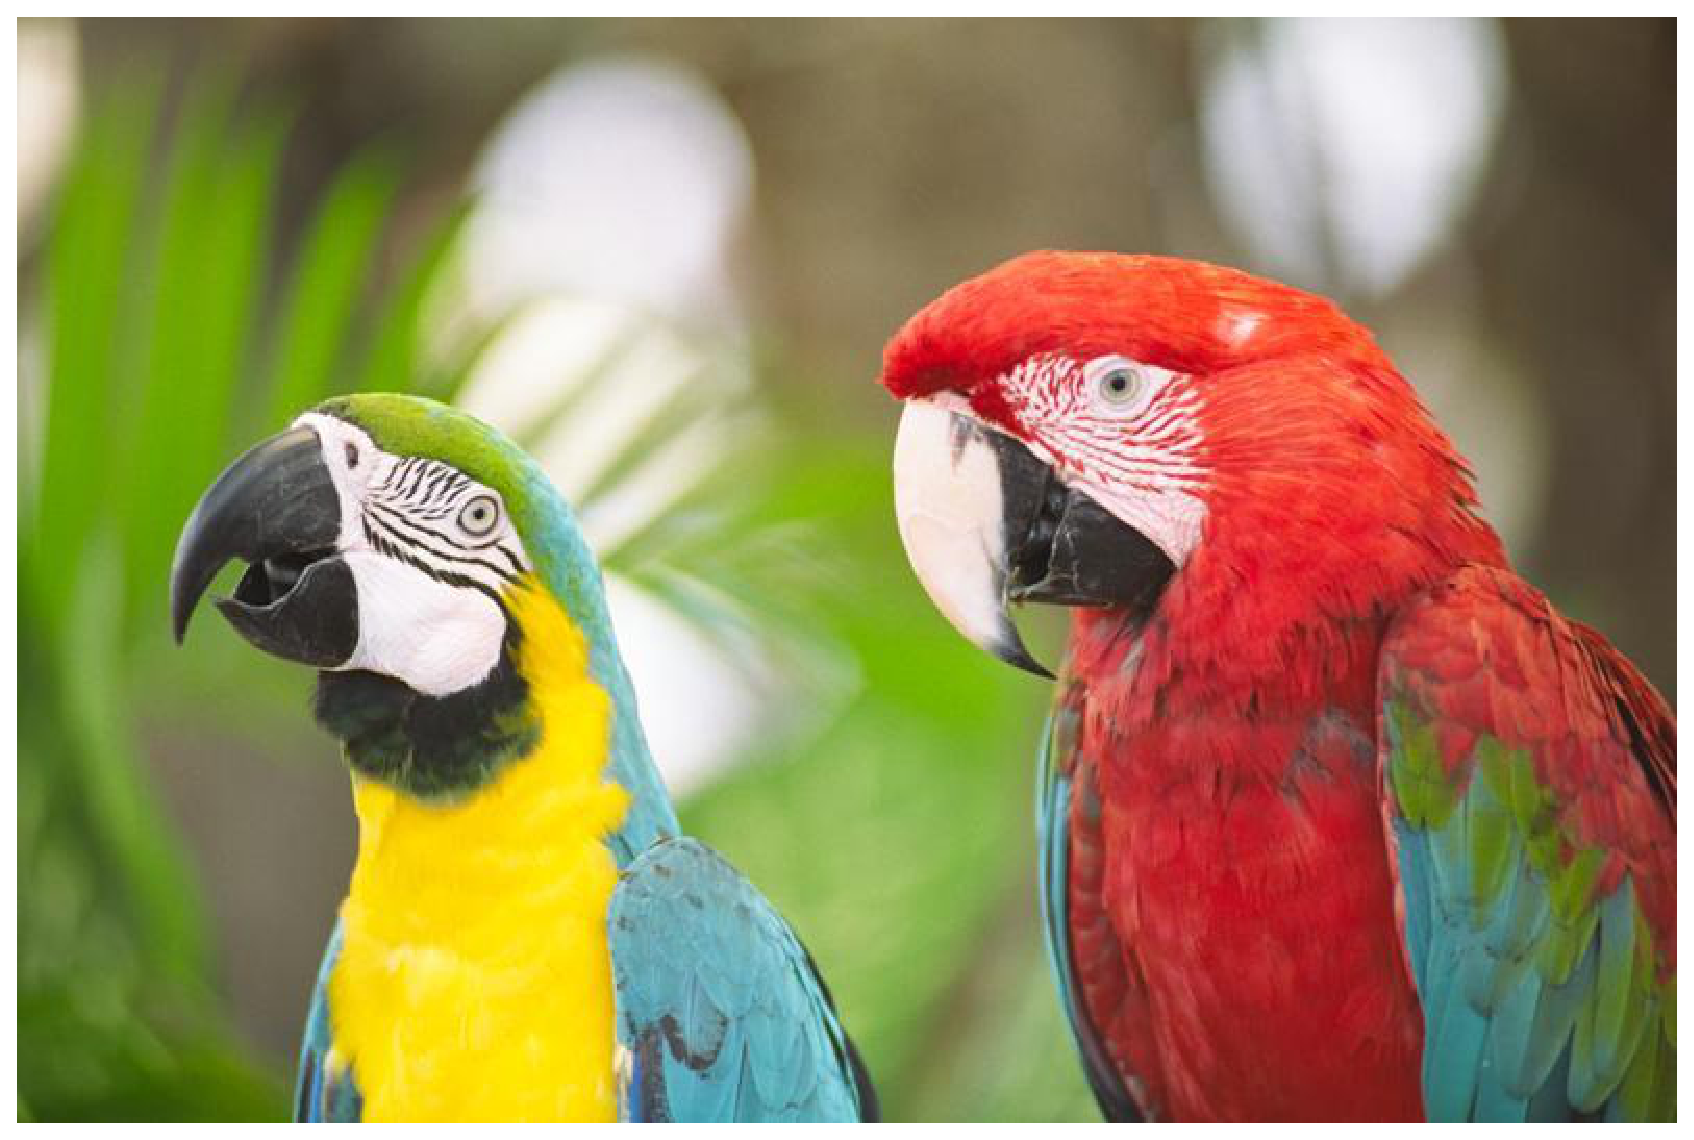
\includegraphics[width=0.24 \textwidth]{bird.eps}}
  \subfloat[][]{\label{figur:2b}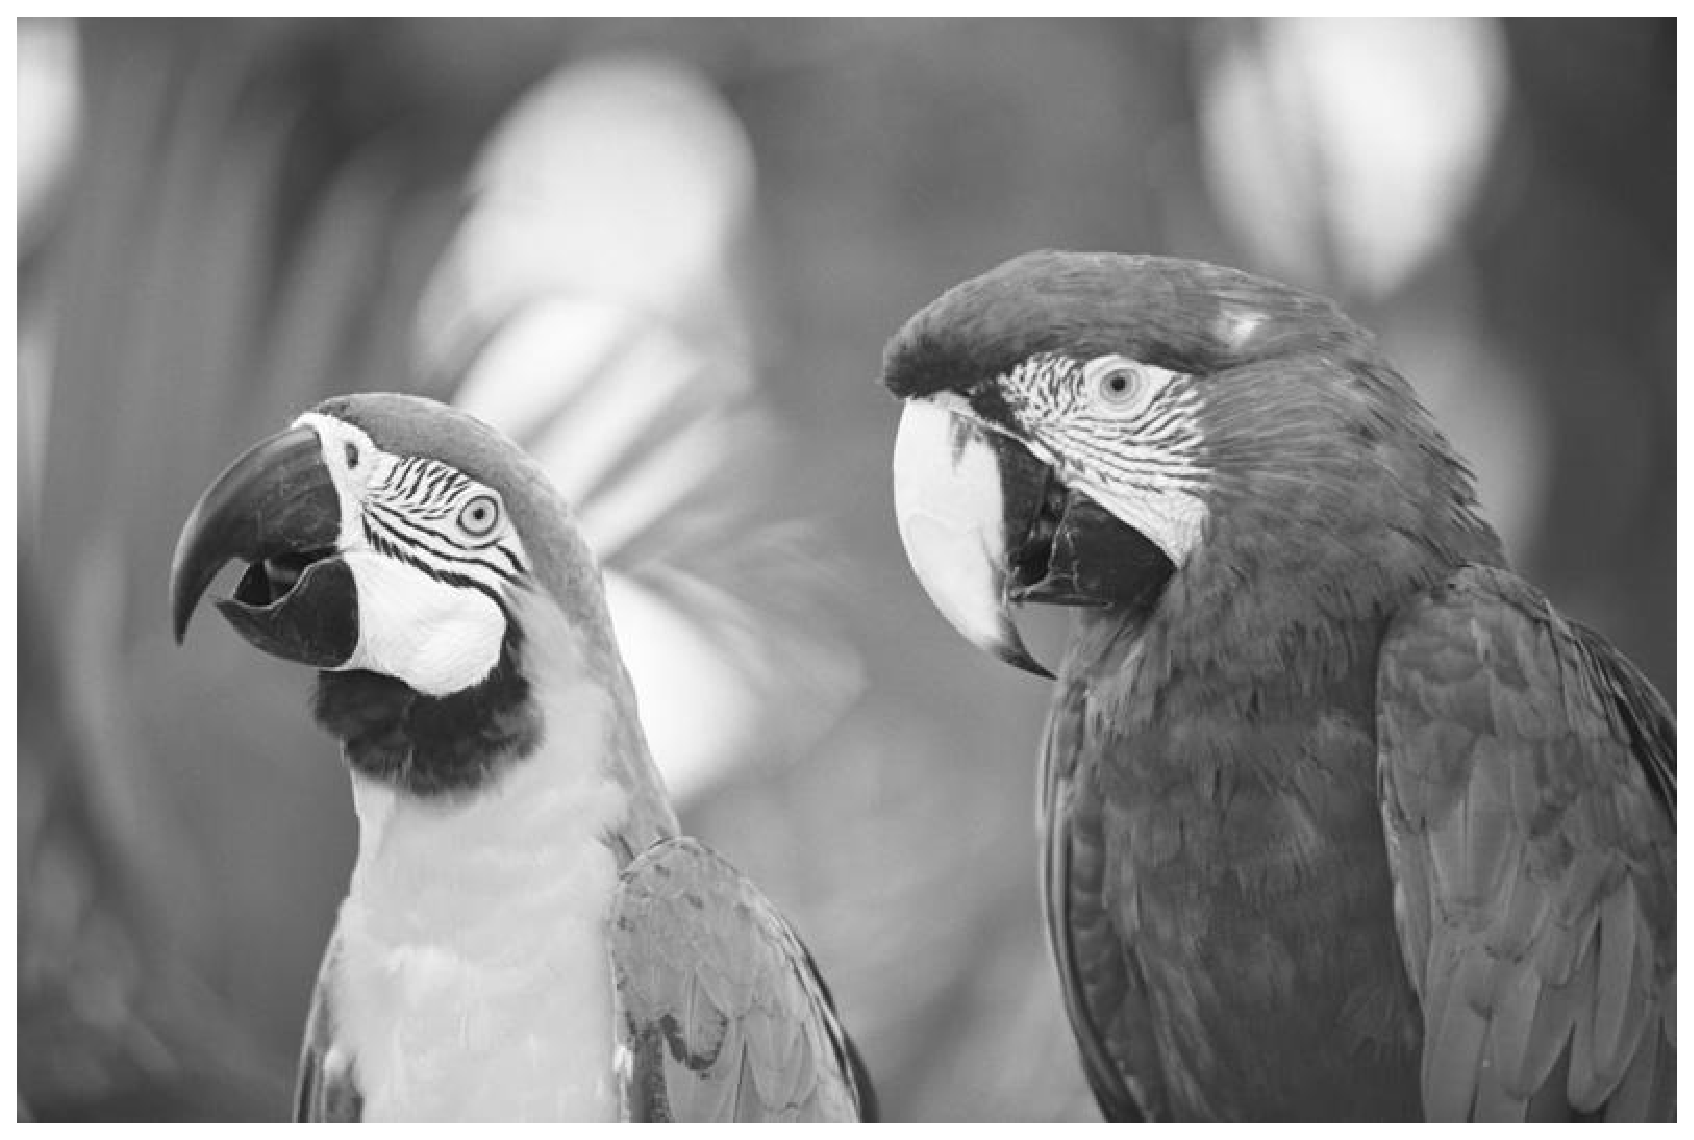
\includegraphics[width=0.24\textwidth]{bird_lum.eps}}
  \\
  \subfloat[][]{\label{figur:2c}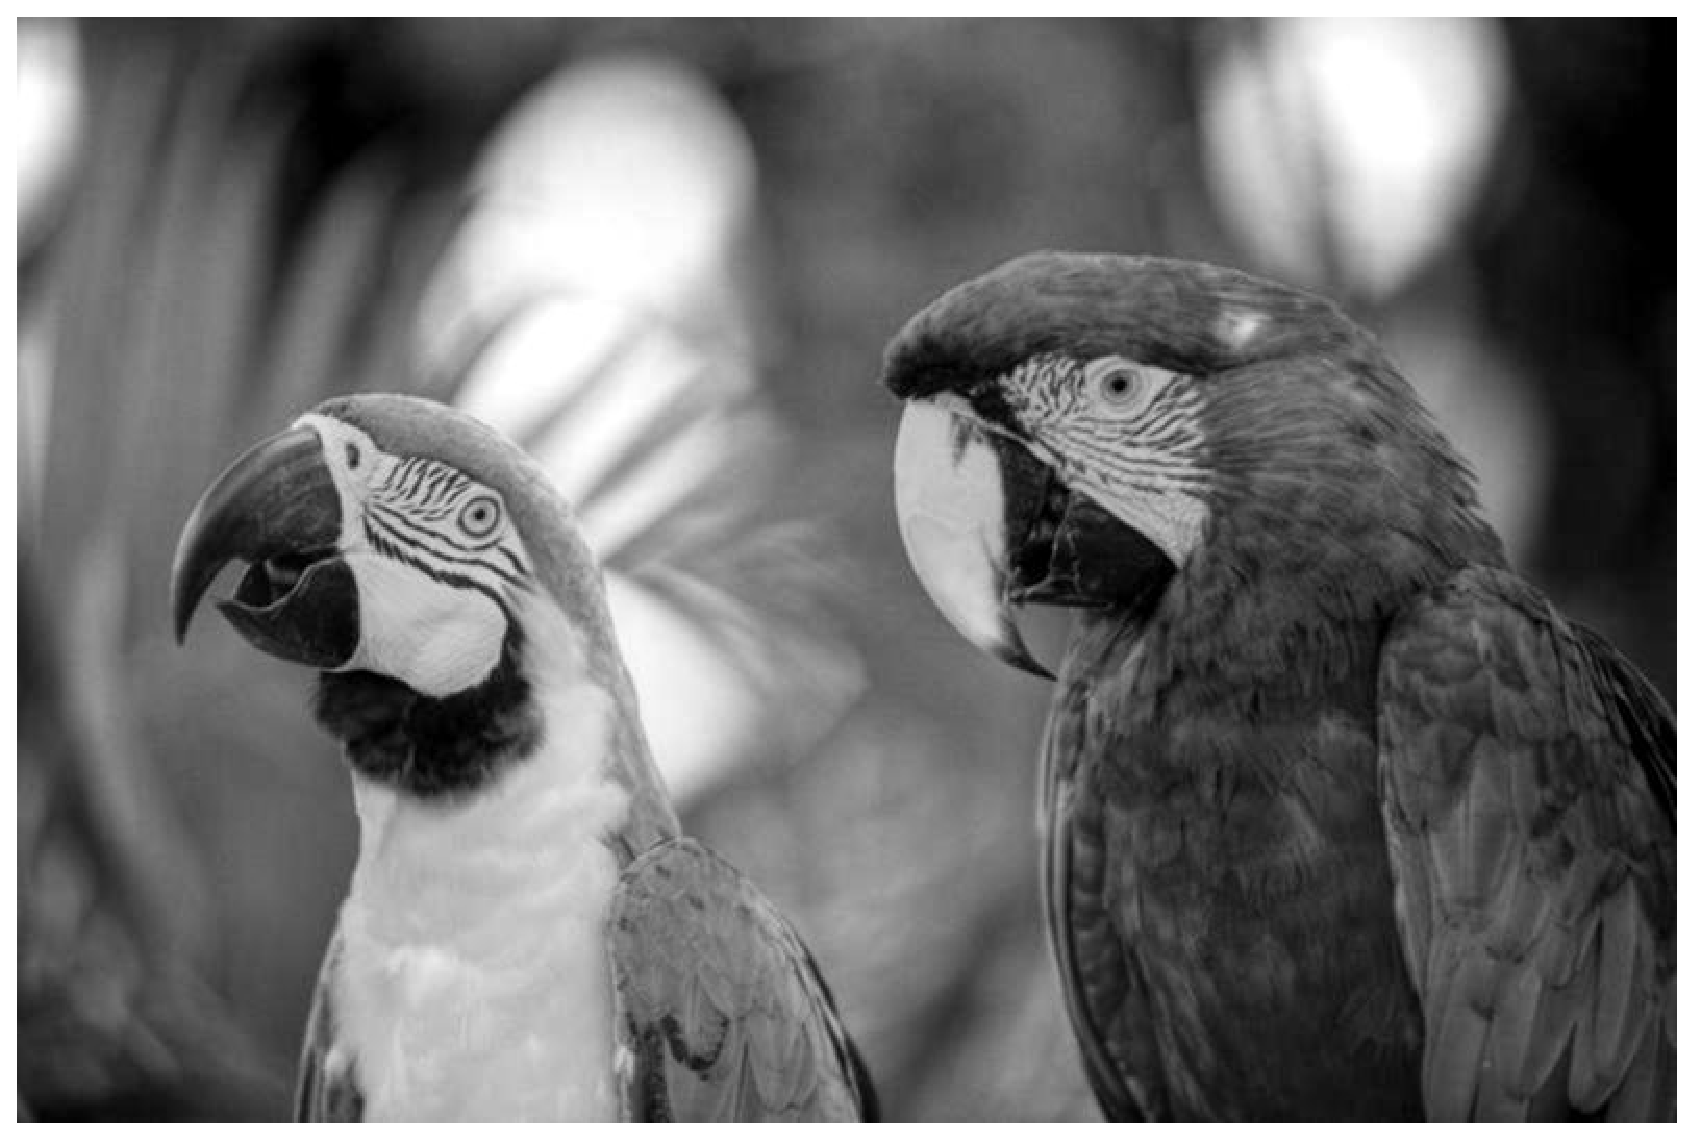
\includegraphics[width=0.24\textwidth]{newMethodBird.eps}}
  \subfloat[][]{\label{figur:2d}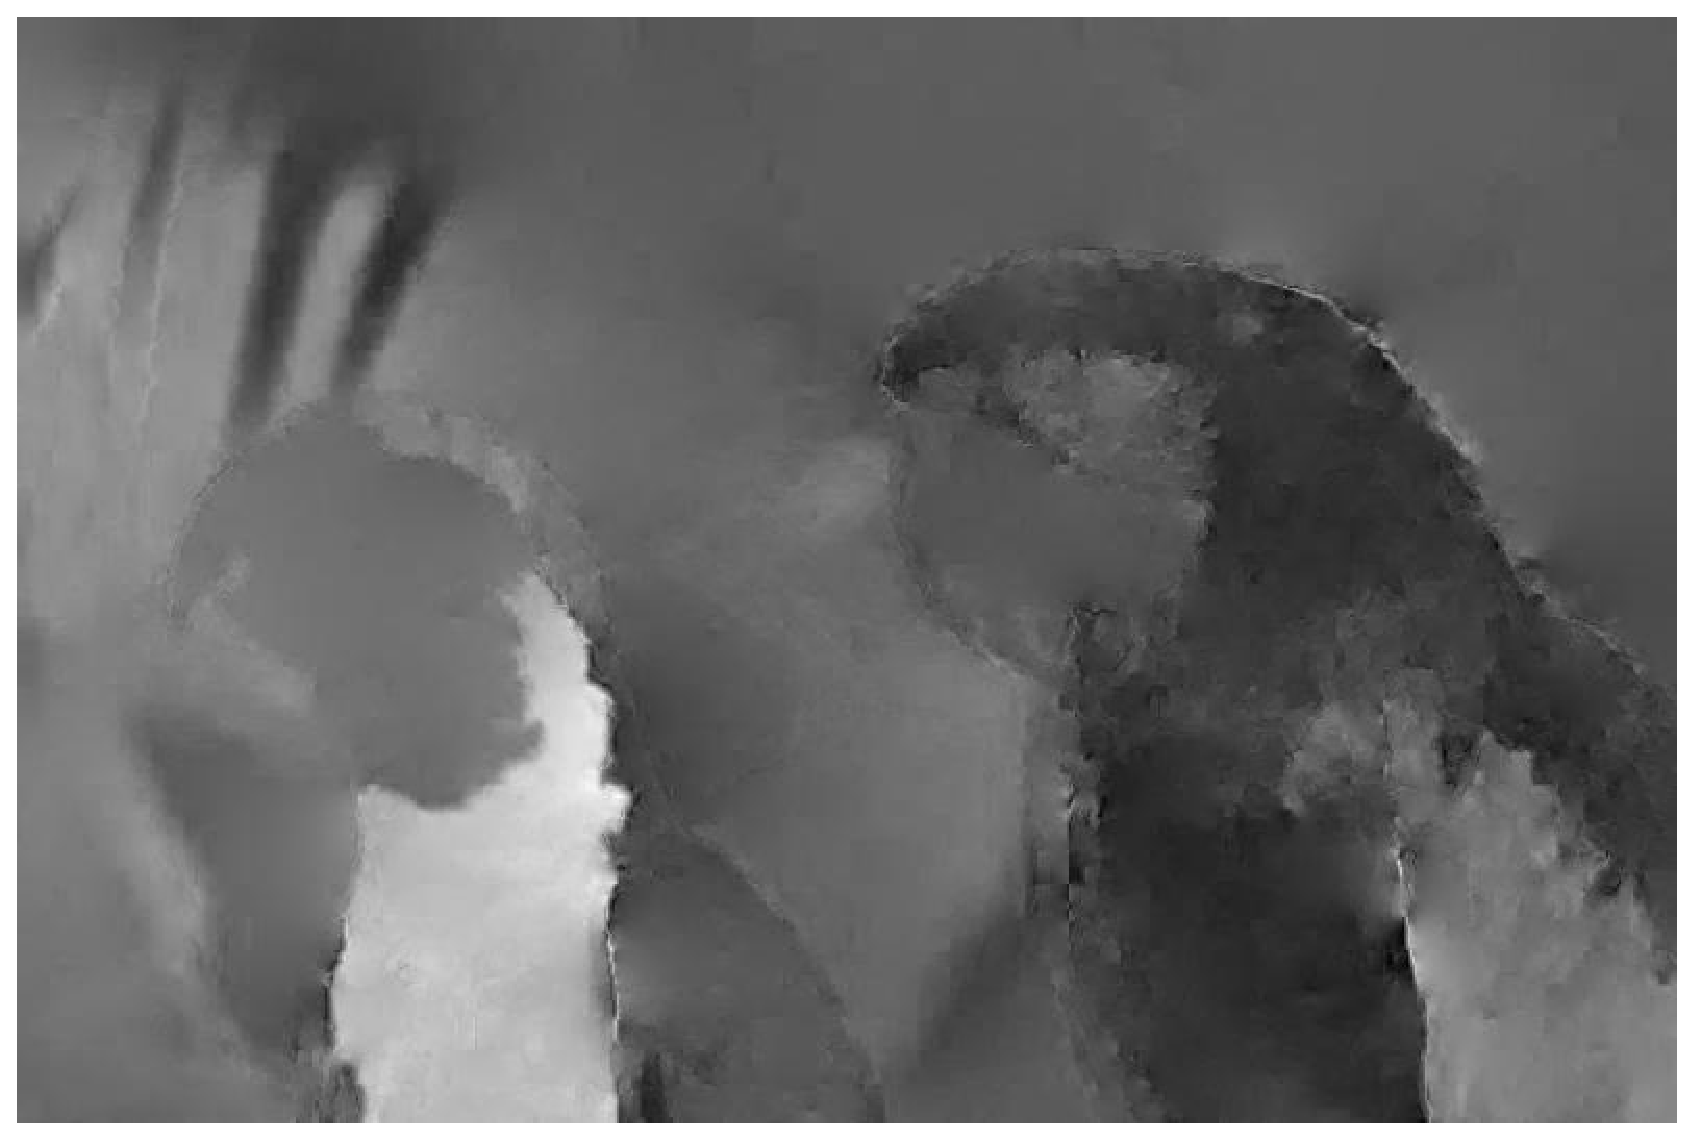
\includegraphics[width=0.24\textwidth]{newMethodBird_rest.eps}}
\caption{Results of converting the parrots original photo~\ref{figur:2a} to grey using the luminance channel~\ref{figur:2b} and the proposed algorithm~\ref{figur:2c}. The results of integrating the leftover gradients are shown in~\ref{figur:2d}.}
\label{fig:2}
\end{figure}
\begin{figure}[t]  
  \centering
  \subfloat[][]{\label{fig:2Lum}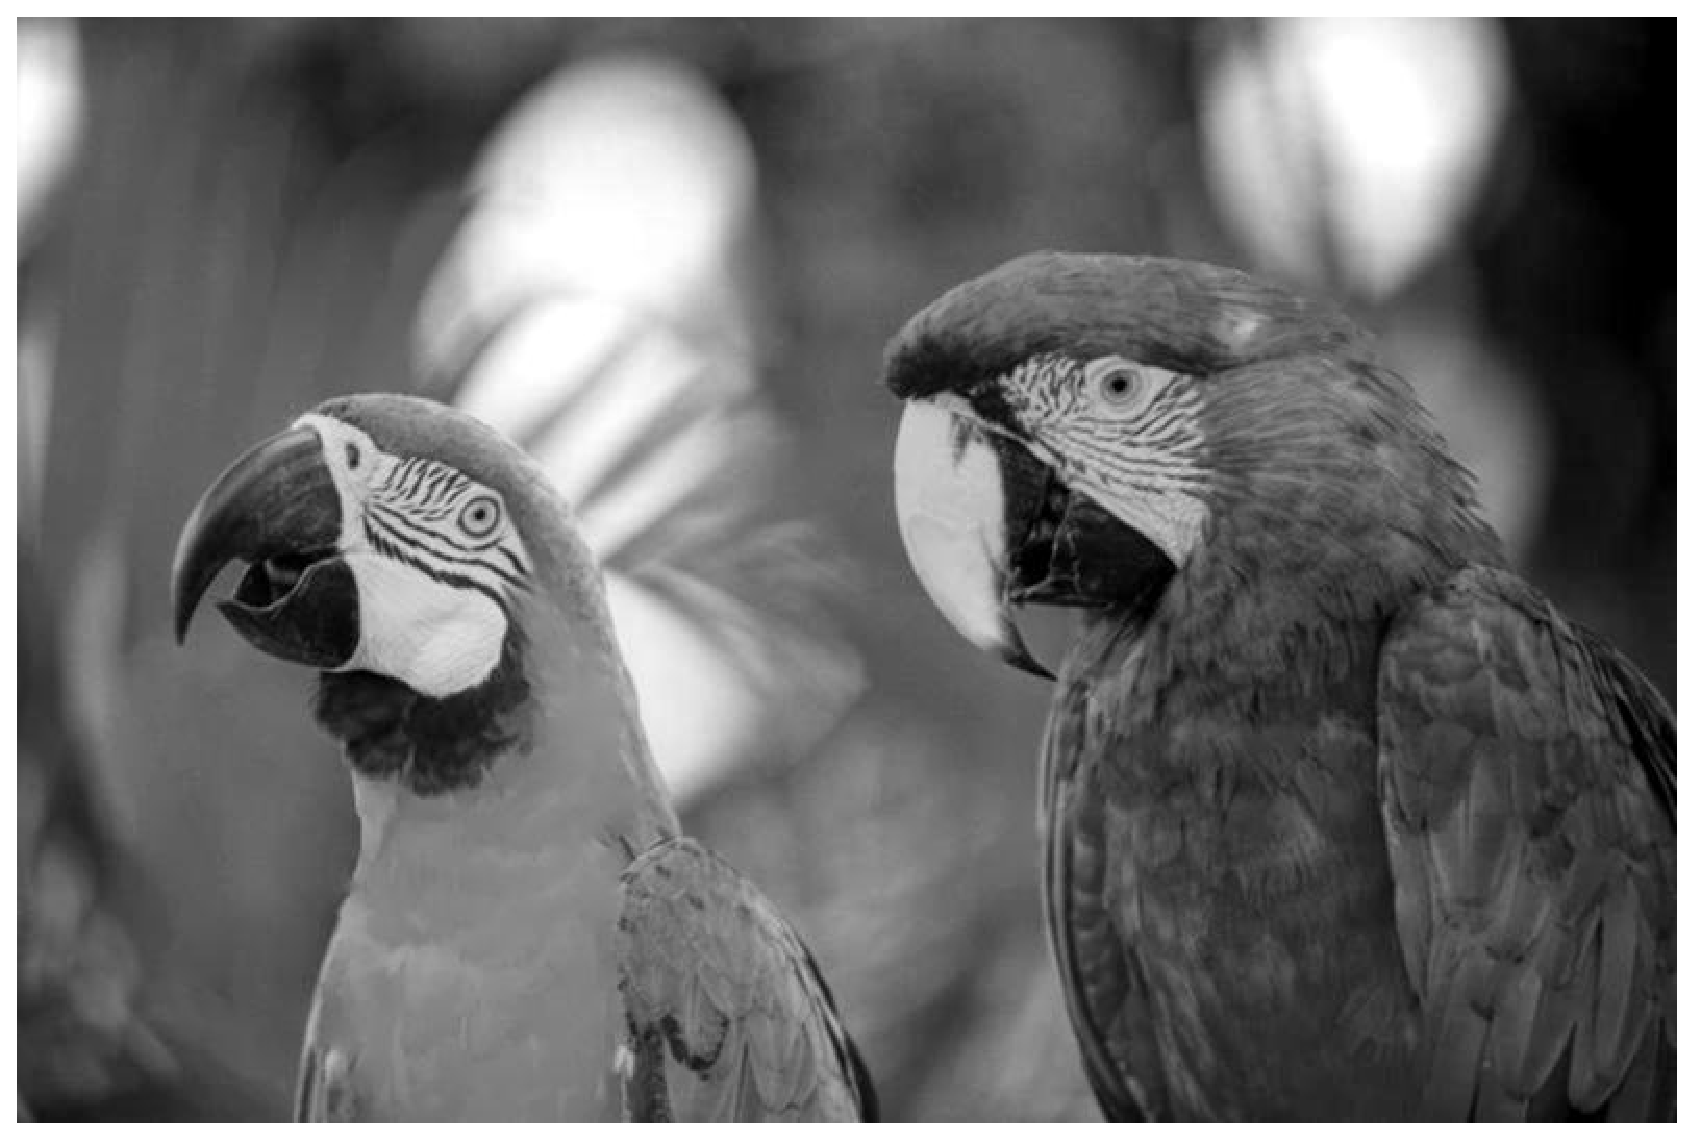
\includegraphics[width=0.24 \textwidth]{newMethodLum.eps}}
  \subfloat[][]{\label{fig:2Chrom}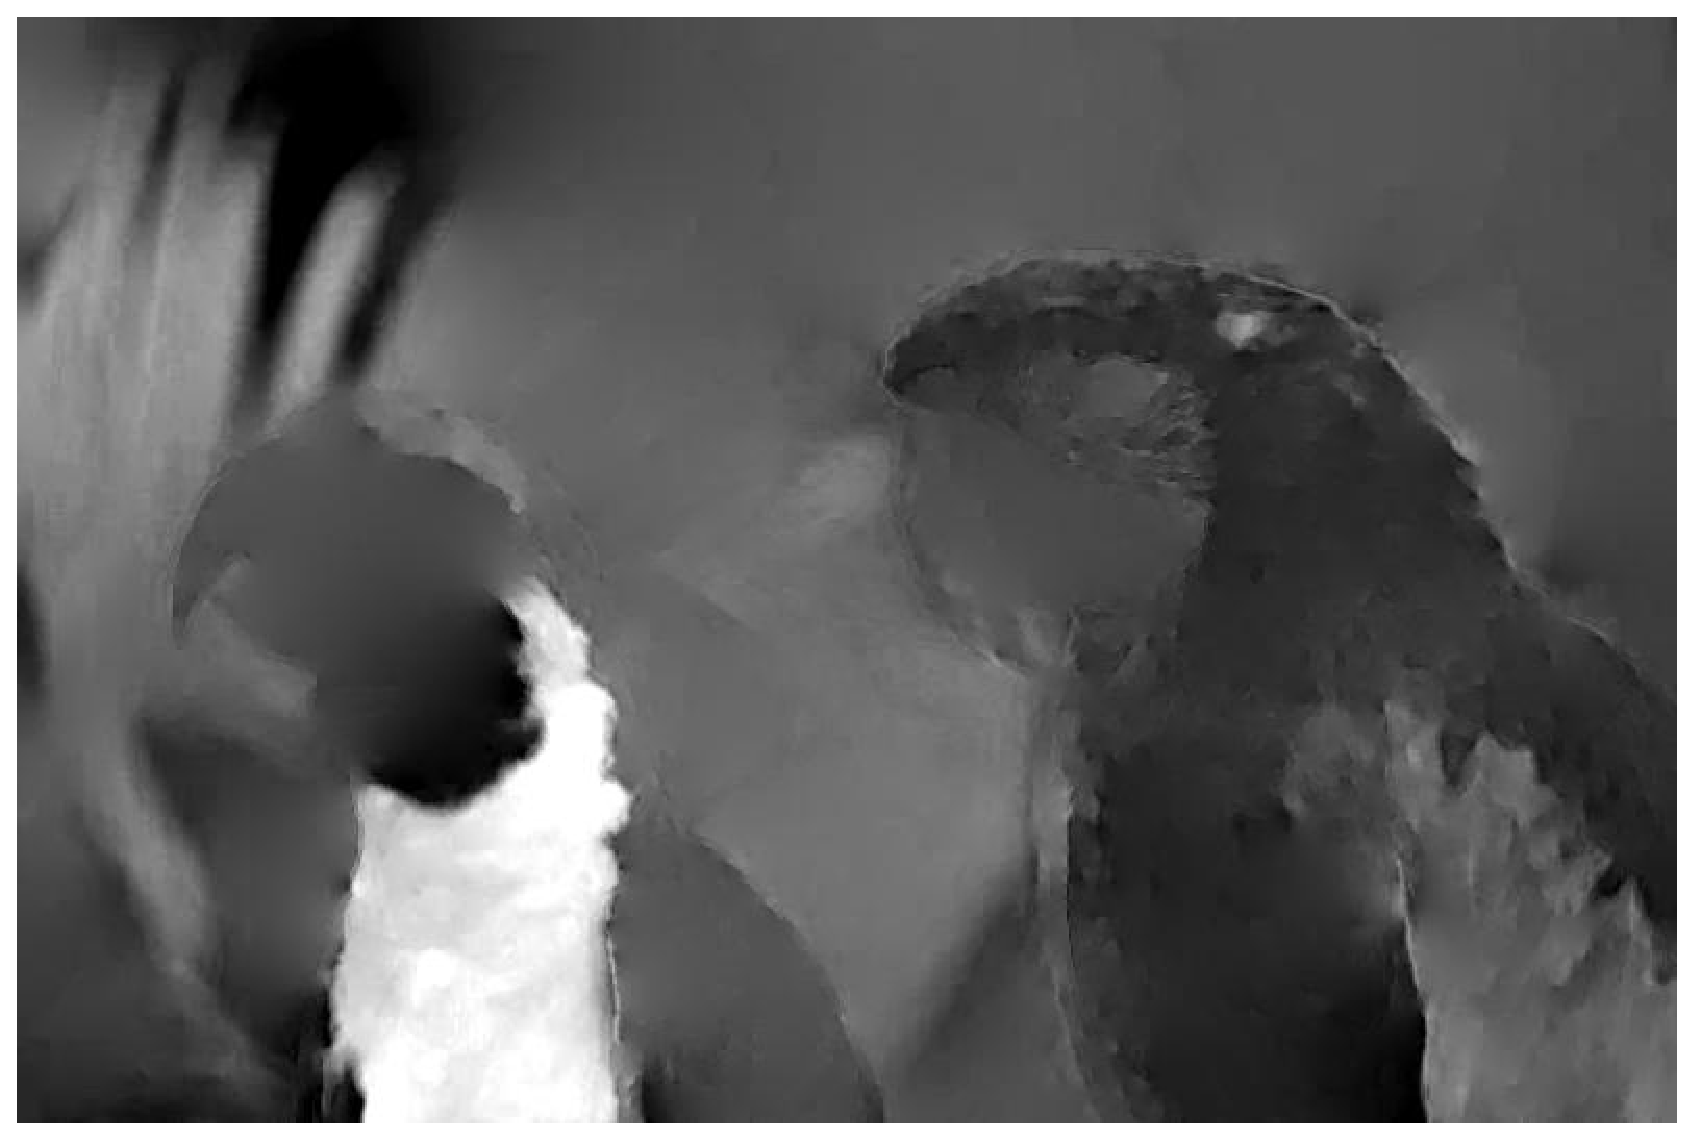
\includegraphics[width=0.24\textwidth]{newMethodChroma.eps}}
\caption{The luminance and chrominance parts of the parrots image~\ref{fig:2Lum} and~\ref{fig:2Chrom} respectively.}
\label{fig:2E}
\end{figure}
\begin{figure}[t]  
  \centering
\psset{xunit=1.2cm,yunit=0.7cm}
\begin{pspicture}(-1,-1)(7,8.5)
\psgrid[gridcolor=gray,subgriddiv=0,gridwidth=0.4pt,gridlabels=0](0,0)(0,0)(6,8)
\pspolygon[linewidth=0.005](0,0)(0,8)(6,8)(6,0)
\rput(0, 0.45033){\color{blue}$\bigstar$}%
\rput(1, 0.44116){\color{blue}$\bigstar$}%
\rput(2, 0.57649){\color{blue}$\bigstar$}%
\rput(3, 0.08842){\color{blue}$\bigstar$}%
\rput(4, 0.31014){\color{blue}$\bigstar$}%
\rput(5, 0.95600){\color{blue}$\bigstar$}%
\rput(6, 7.14831){\color{blue}$\bigstar$}%
\rput[r](-0.1,0){\scriptsize 0.0}%
\rput[r](-0.1,1){\scriptsize 0.1}%
\rput[r](-0.1,2){\scriptsize 0.2}%
\rput[r](-0.1,3){\scriptsize 0.3}%
\rput[r](-0.1,4){\scriptsize 0.4}%
\rput[r](-0.1,5){\scriptsize 0.5}%
\rput[r](-0.1,6){\scriptsize 0.6}%
\rput[r](-0.1,7){\scriptsize 0.7}%
\rput[r](-0.1,8){\scriptsize 0.8}%
\rput[B](0,-0.40){\scriptsize blue}%
\rput[B](1,-0.40){\scriptsize green}%
\rput[B](2,-0.40){\scriptsize cyan}%
\rput[B](3,-0.40){\scriptsize red}%
\rput[B](4,-0.40){\scriptsize magenta}%
\rput[B](5,-0.40){\scriptsize yellow}%
\rput[B](6,-0.40){\scriptsize white}%
\rput[B](3,-0.96){Maximum gradient direction}%
\rput{90}(-.6,4){Normalised count}%
\end{pspicture}
%{\includegraphics[width=0.47\textwidth]{gradients_bird2.eps}}
\caption{The percentage of maximum signed gradients for the arrots image in different directions. Here white is luminance gradients and it is the direction in which all the colour values increase or decrease.}
\label{fig:2G}
\end{figure}
In figure~\ref{fig:3}, we show the results obtained for five colour caps. Similar to the parrots image, we observe that the results of the proposed algorithm, figure~\ref{figur:3c} exhibit more local contrast than those obtained by the direct luminance method, figure~\ref{figur:3b}.
More, interestingly the result of integrating the leftover gradients into an image~\ref{figur:3d}  shows less information loss than what was obtained from the parrot image figure~\ref{figur:2d}.
In the case of the caps, the leftover gradients contain visual information that allow an observer to detect the contours of the yellow and orange caps but much less so of the other three.
These results bring us to conclude that there are two types of chrominance edges: one where the different channels have opposing directions and another where one or more channels has zero change. The latter case produces zero leftover gradients while the former divides the gradients into negative and positive parts. The proposed algorithm chooses the greatest. 
\begin{figure}[t]  
  \centering
  \subfloat[][]{\label{figur:3a}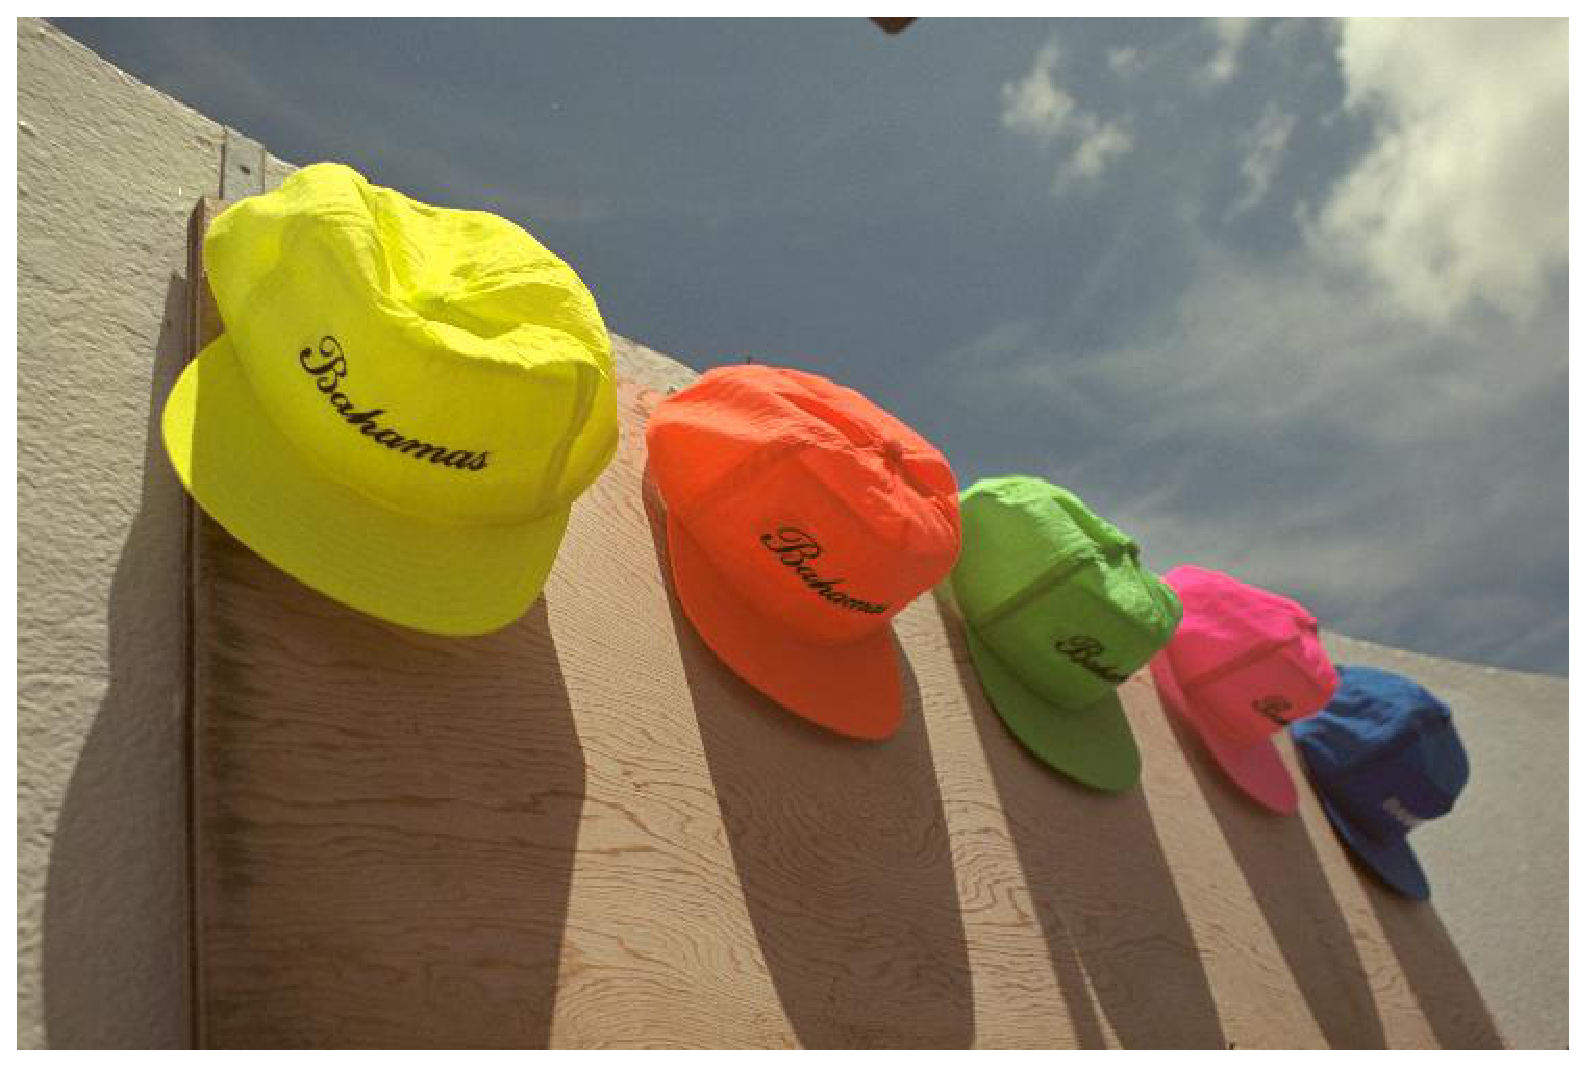
\includegraphics[width=0.24 \textwidth]{caps.eps}}
  \subfloat[][]{\label{figur:3b}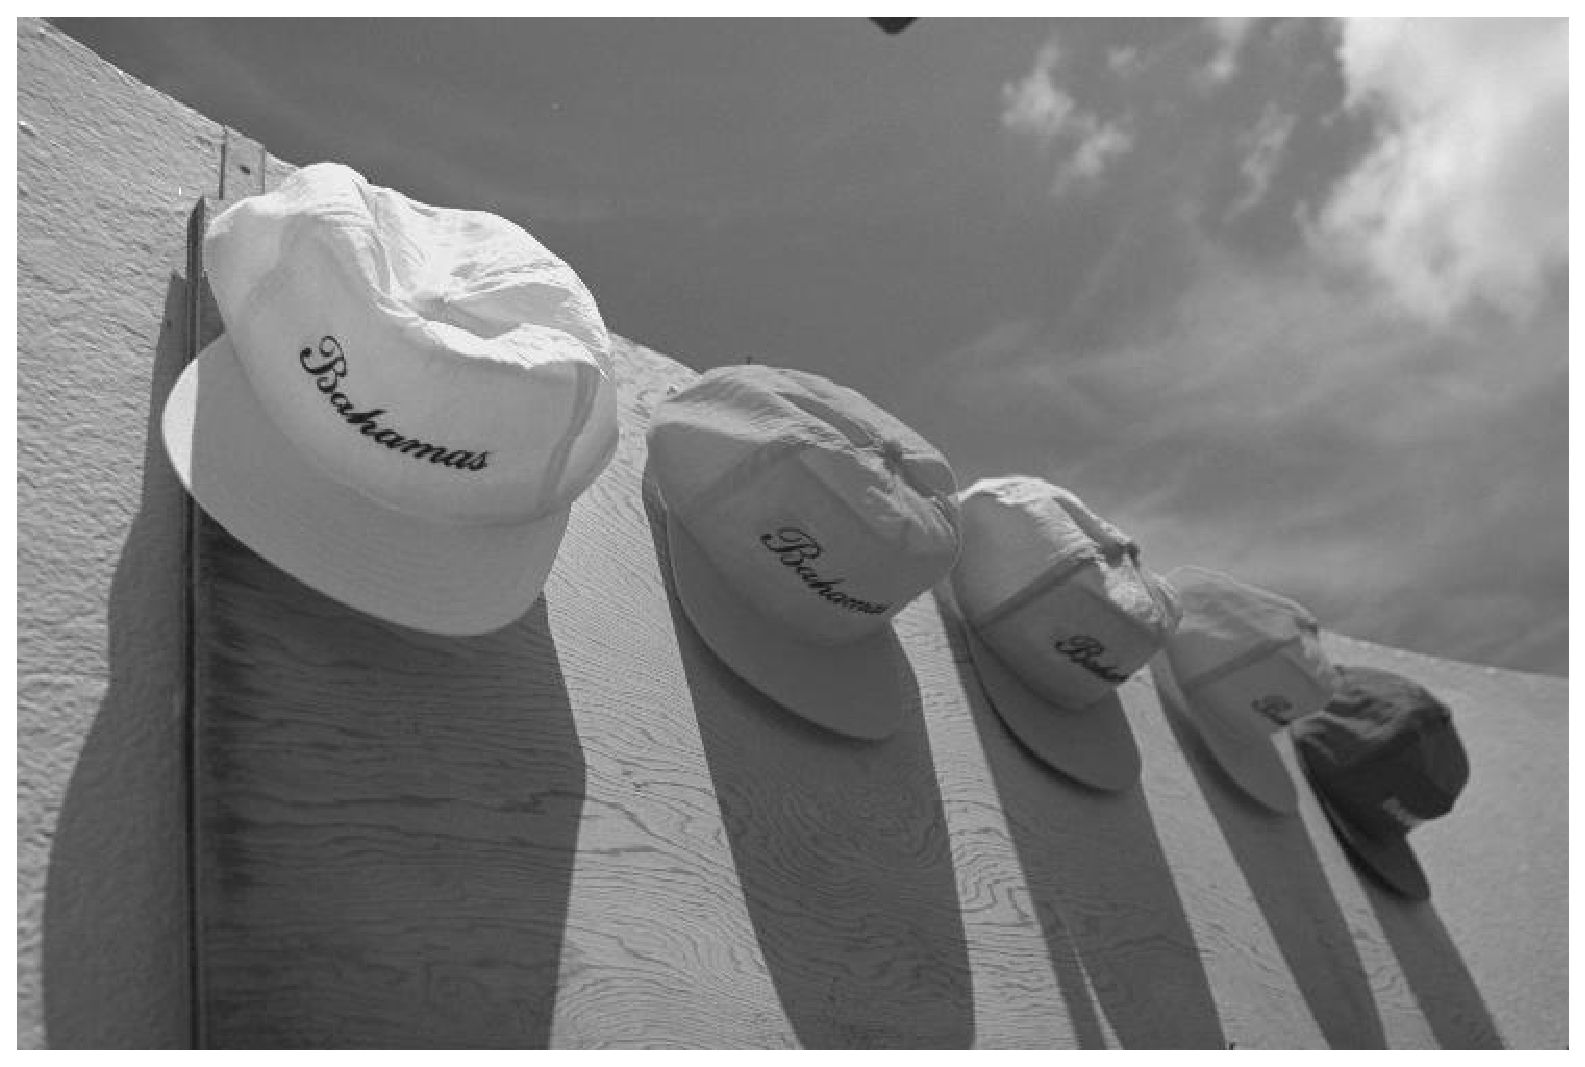
\includegraphics[width=0.24\textwidth]{caps_lum.eps}}
  \\
  \subfloat[][]{\label{figur:3c}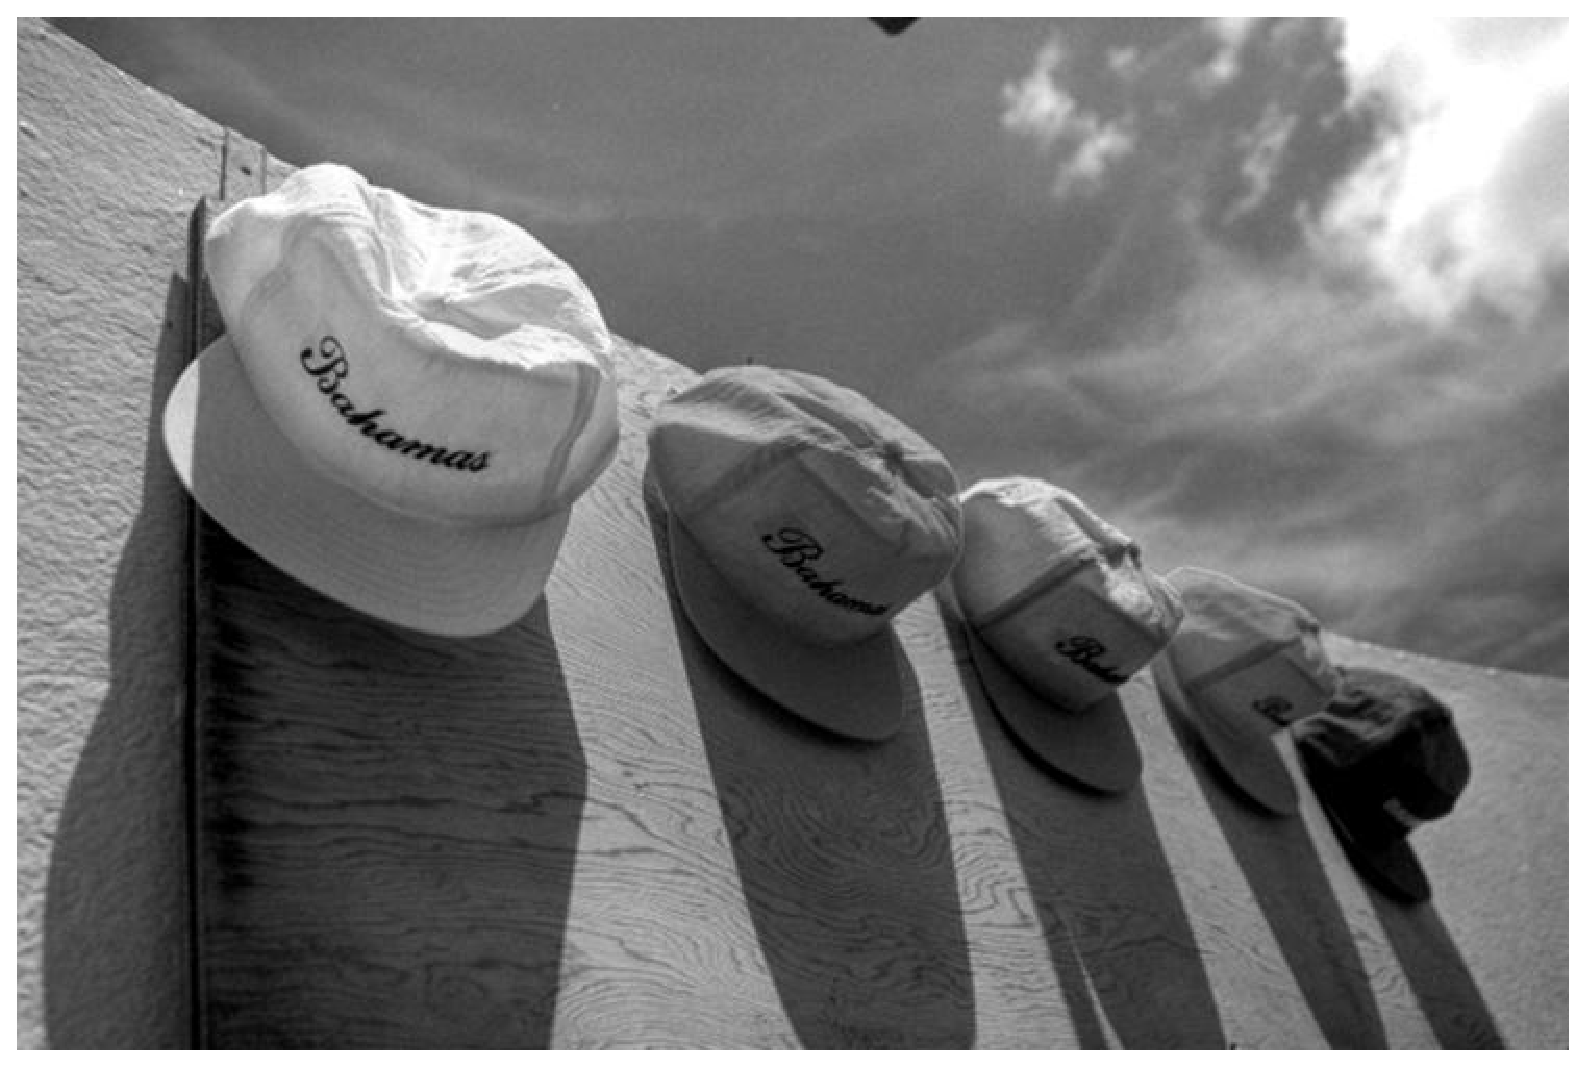
\includegraphics[width=0.24\textwidth]{newMethodCaps.eps}}
  \subfloat[][]{\label{figur:3d}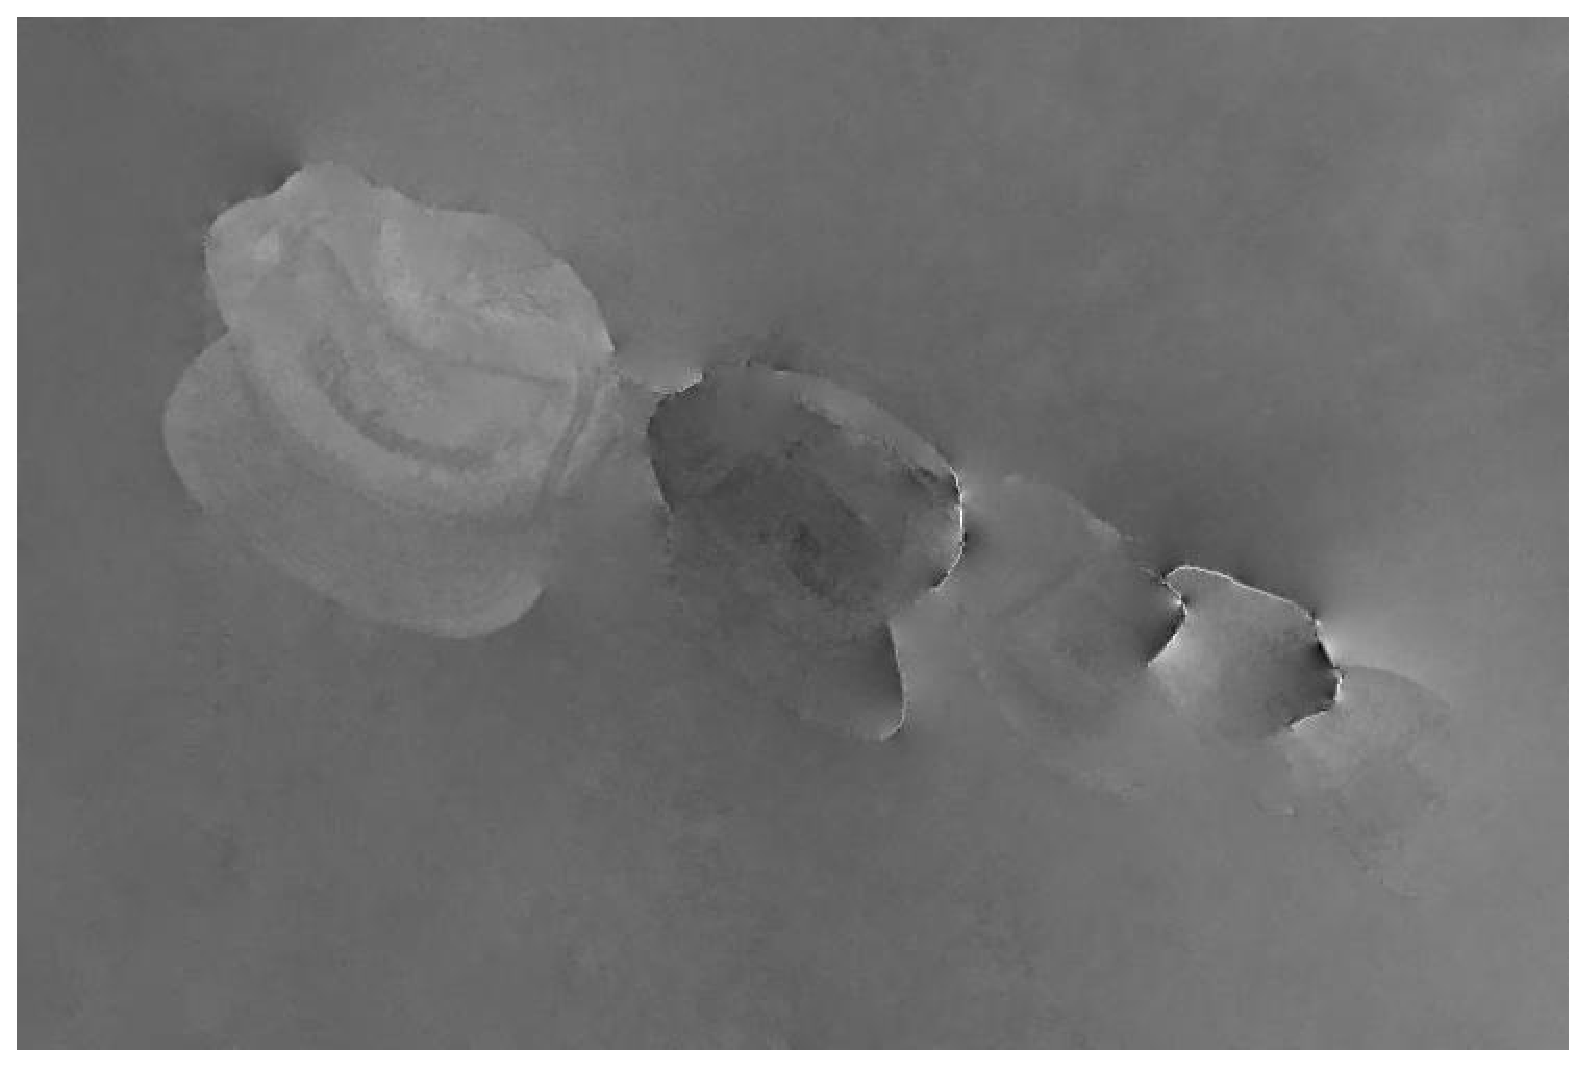
\includegraphics[width=0.24\textwidth]{newMethodCaps_rest.eps}}
\caption{Results of converting the caps' original photo~\ref{figur:3a} to grey using the luminance channel~\ref{figur:3b} and the proposed algorithm~\ref{figur:3c}. The results of integrating the leftover gradients are shown in~\ref{figur:3d}.}
\label{fig:3}
\end{figure}
The last image depicts the Hungarian Parliament building in Budapest. Here, the proposed method results in high local contrast when compared to the luminance projection. The interesting difference is, however, that the leftover gradient, figure~\ref{figur:4d} produces no discernible elements. 
\begin{figure}[t]  
  \centering
  \subfloat[][]{\label{figur:4a}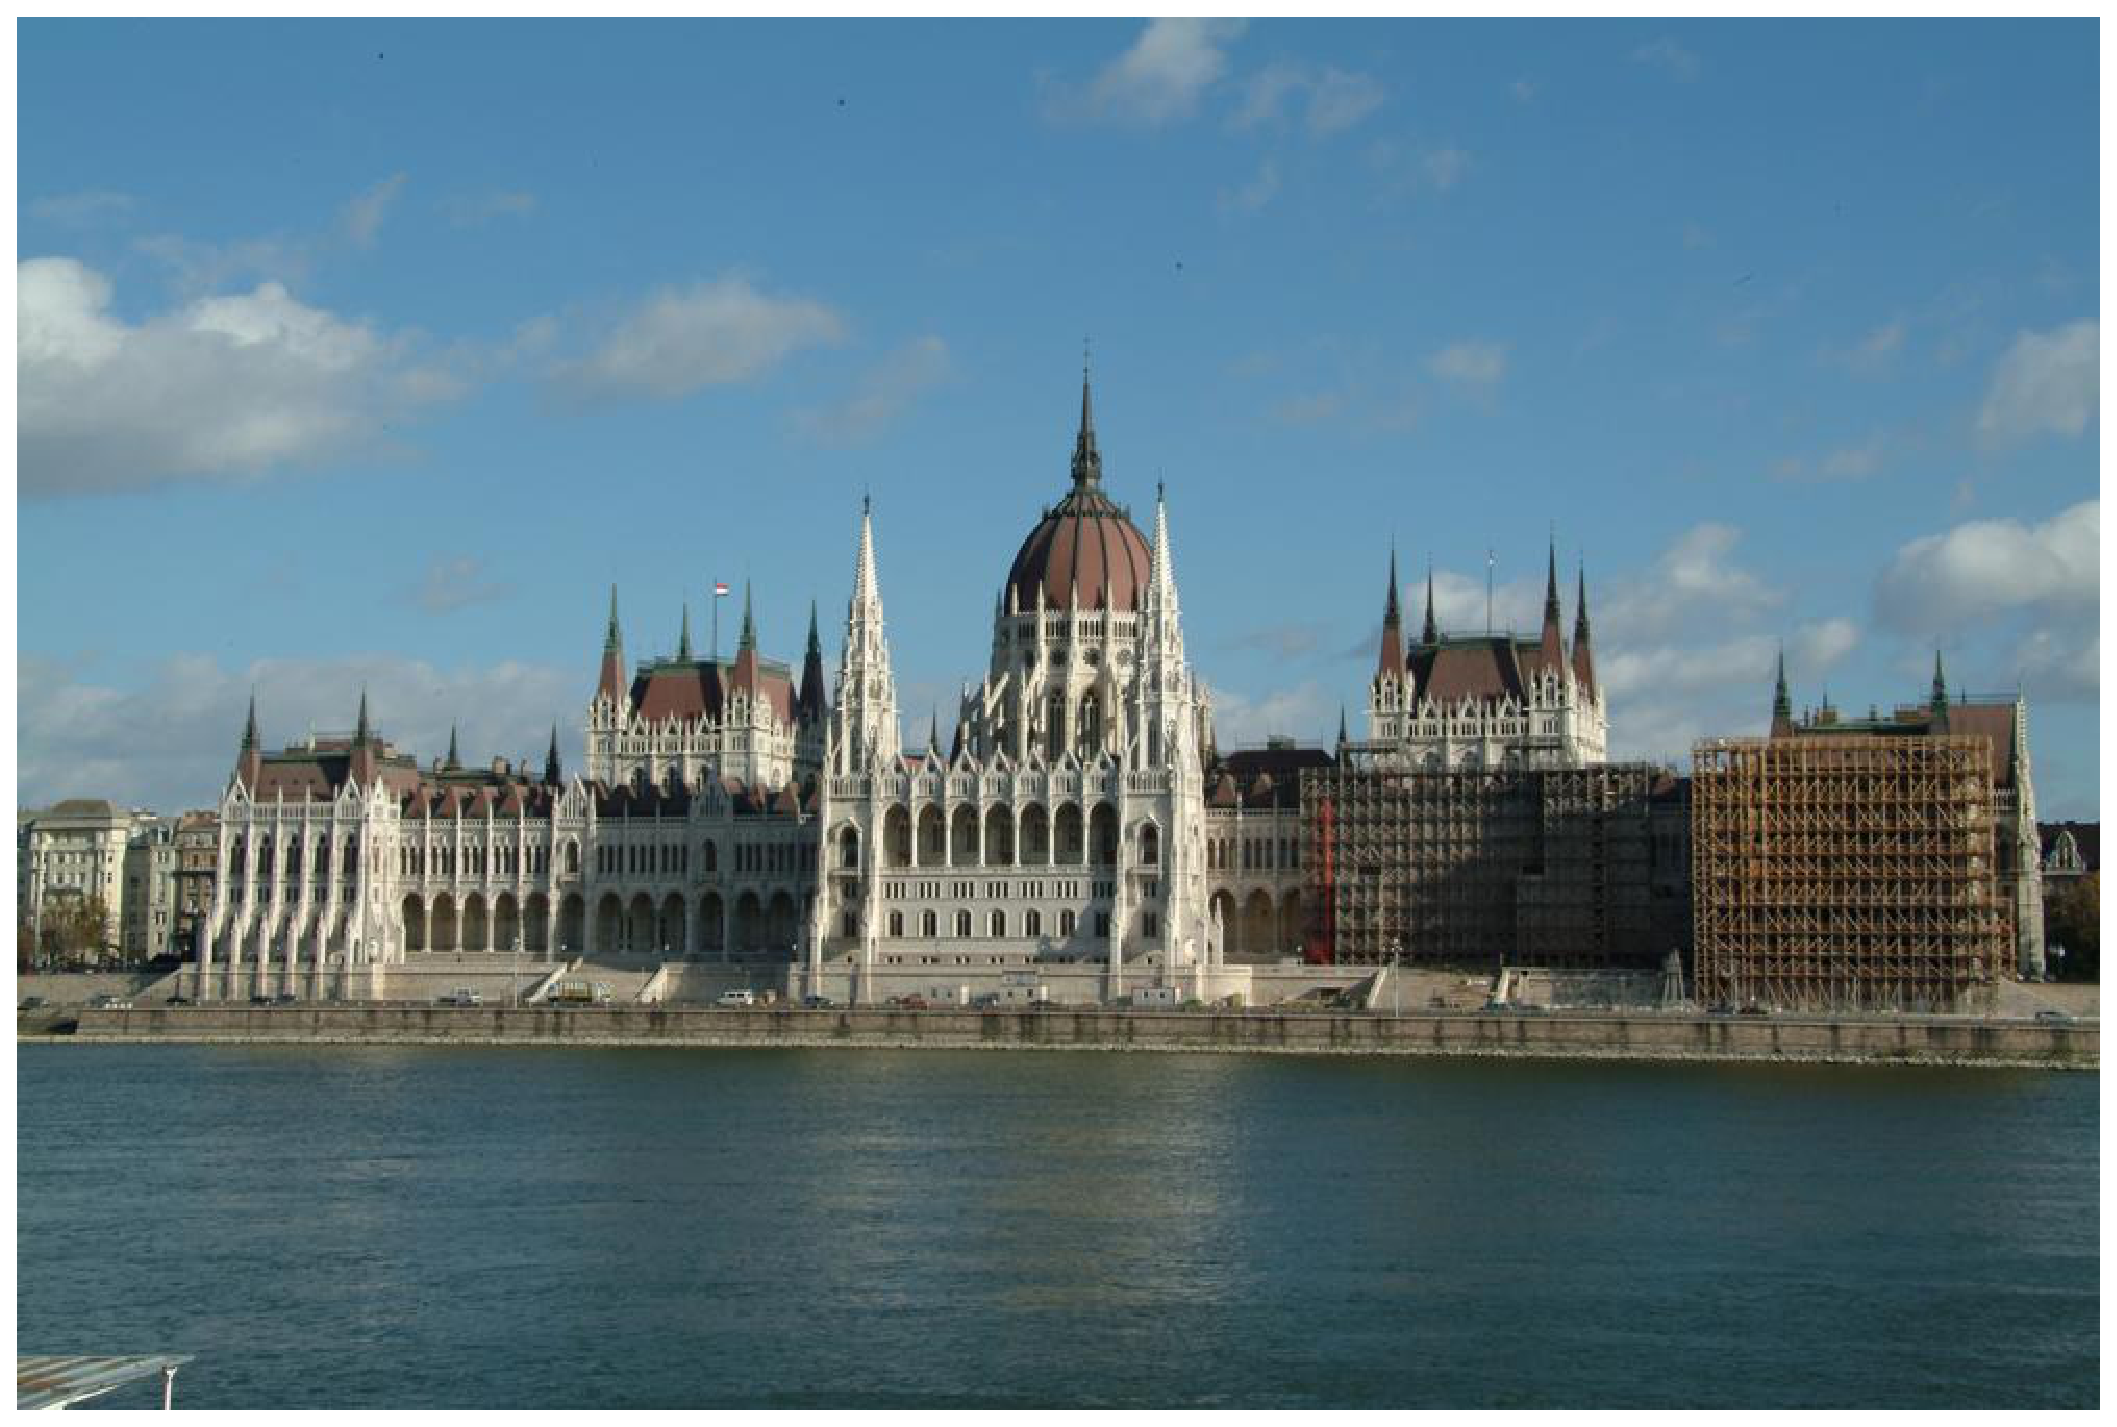
\includegraphics[width=0.24 \textwidth]{buda.eps}}
  \subfloat[][]{\label{figur:4b}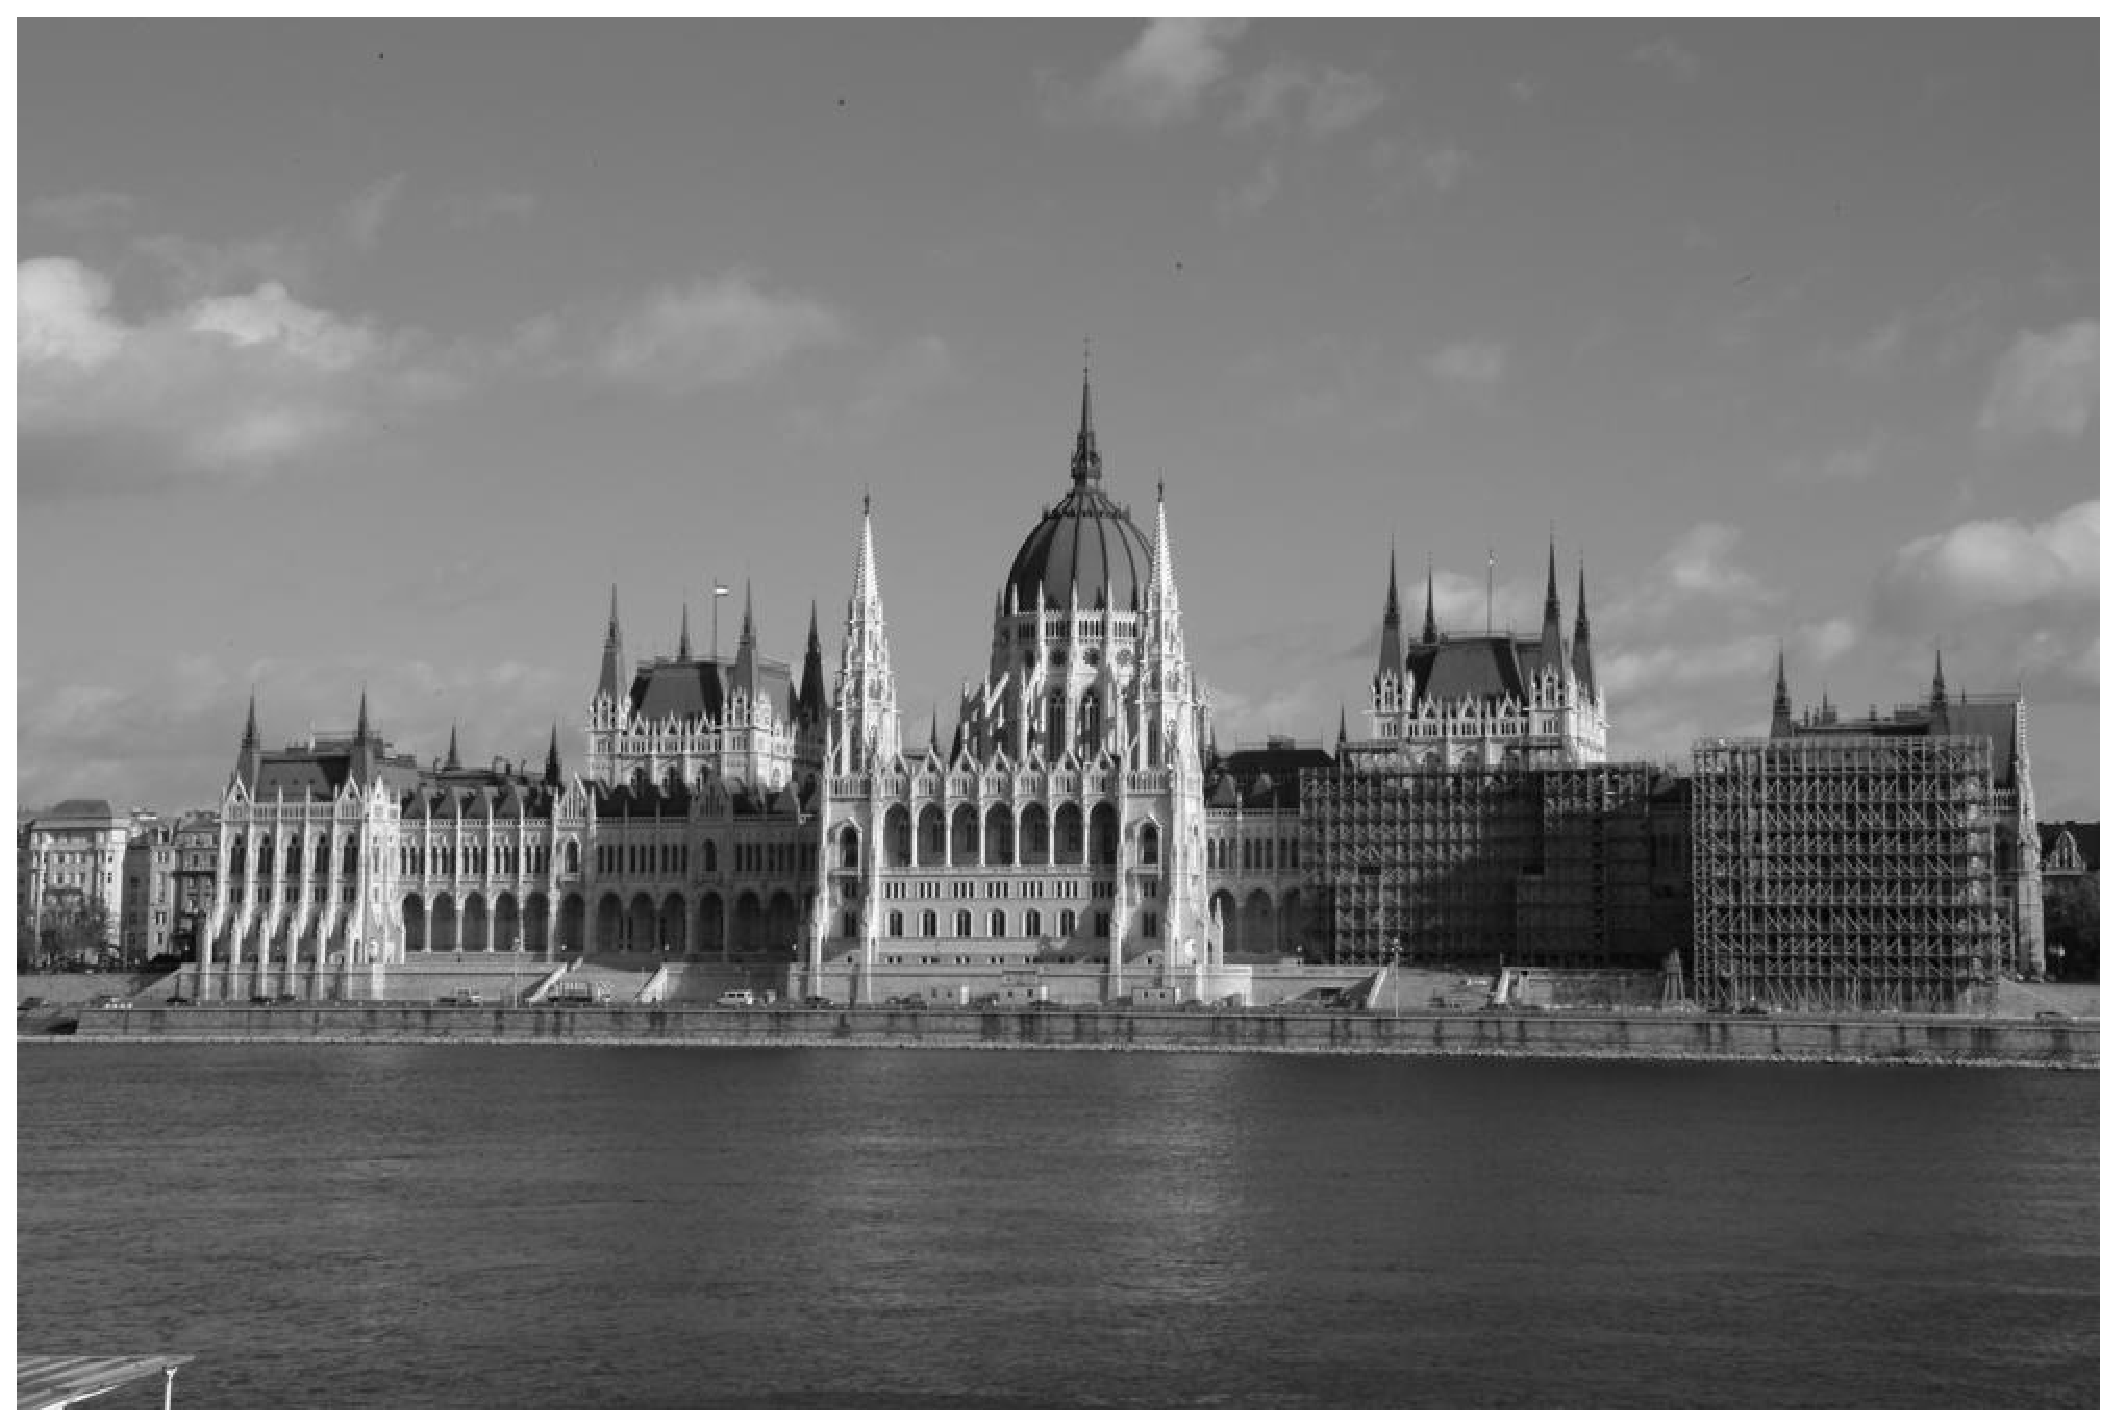
\includegraphics[width=0.24\textwidth]{buda_lum.eps}}
  \\
  \subfloat[][]{\label{figur:4c}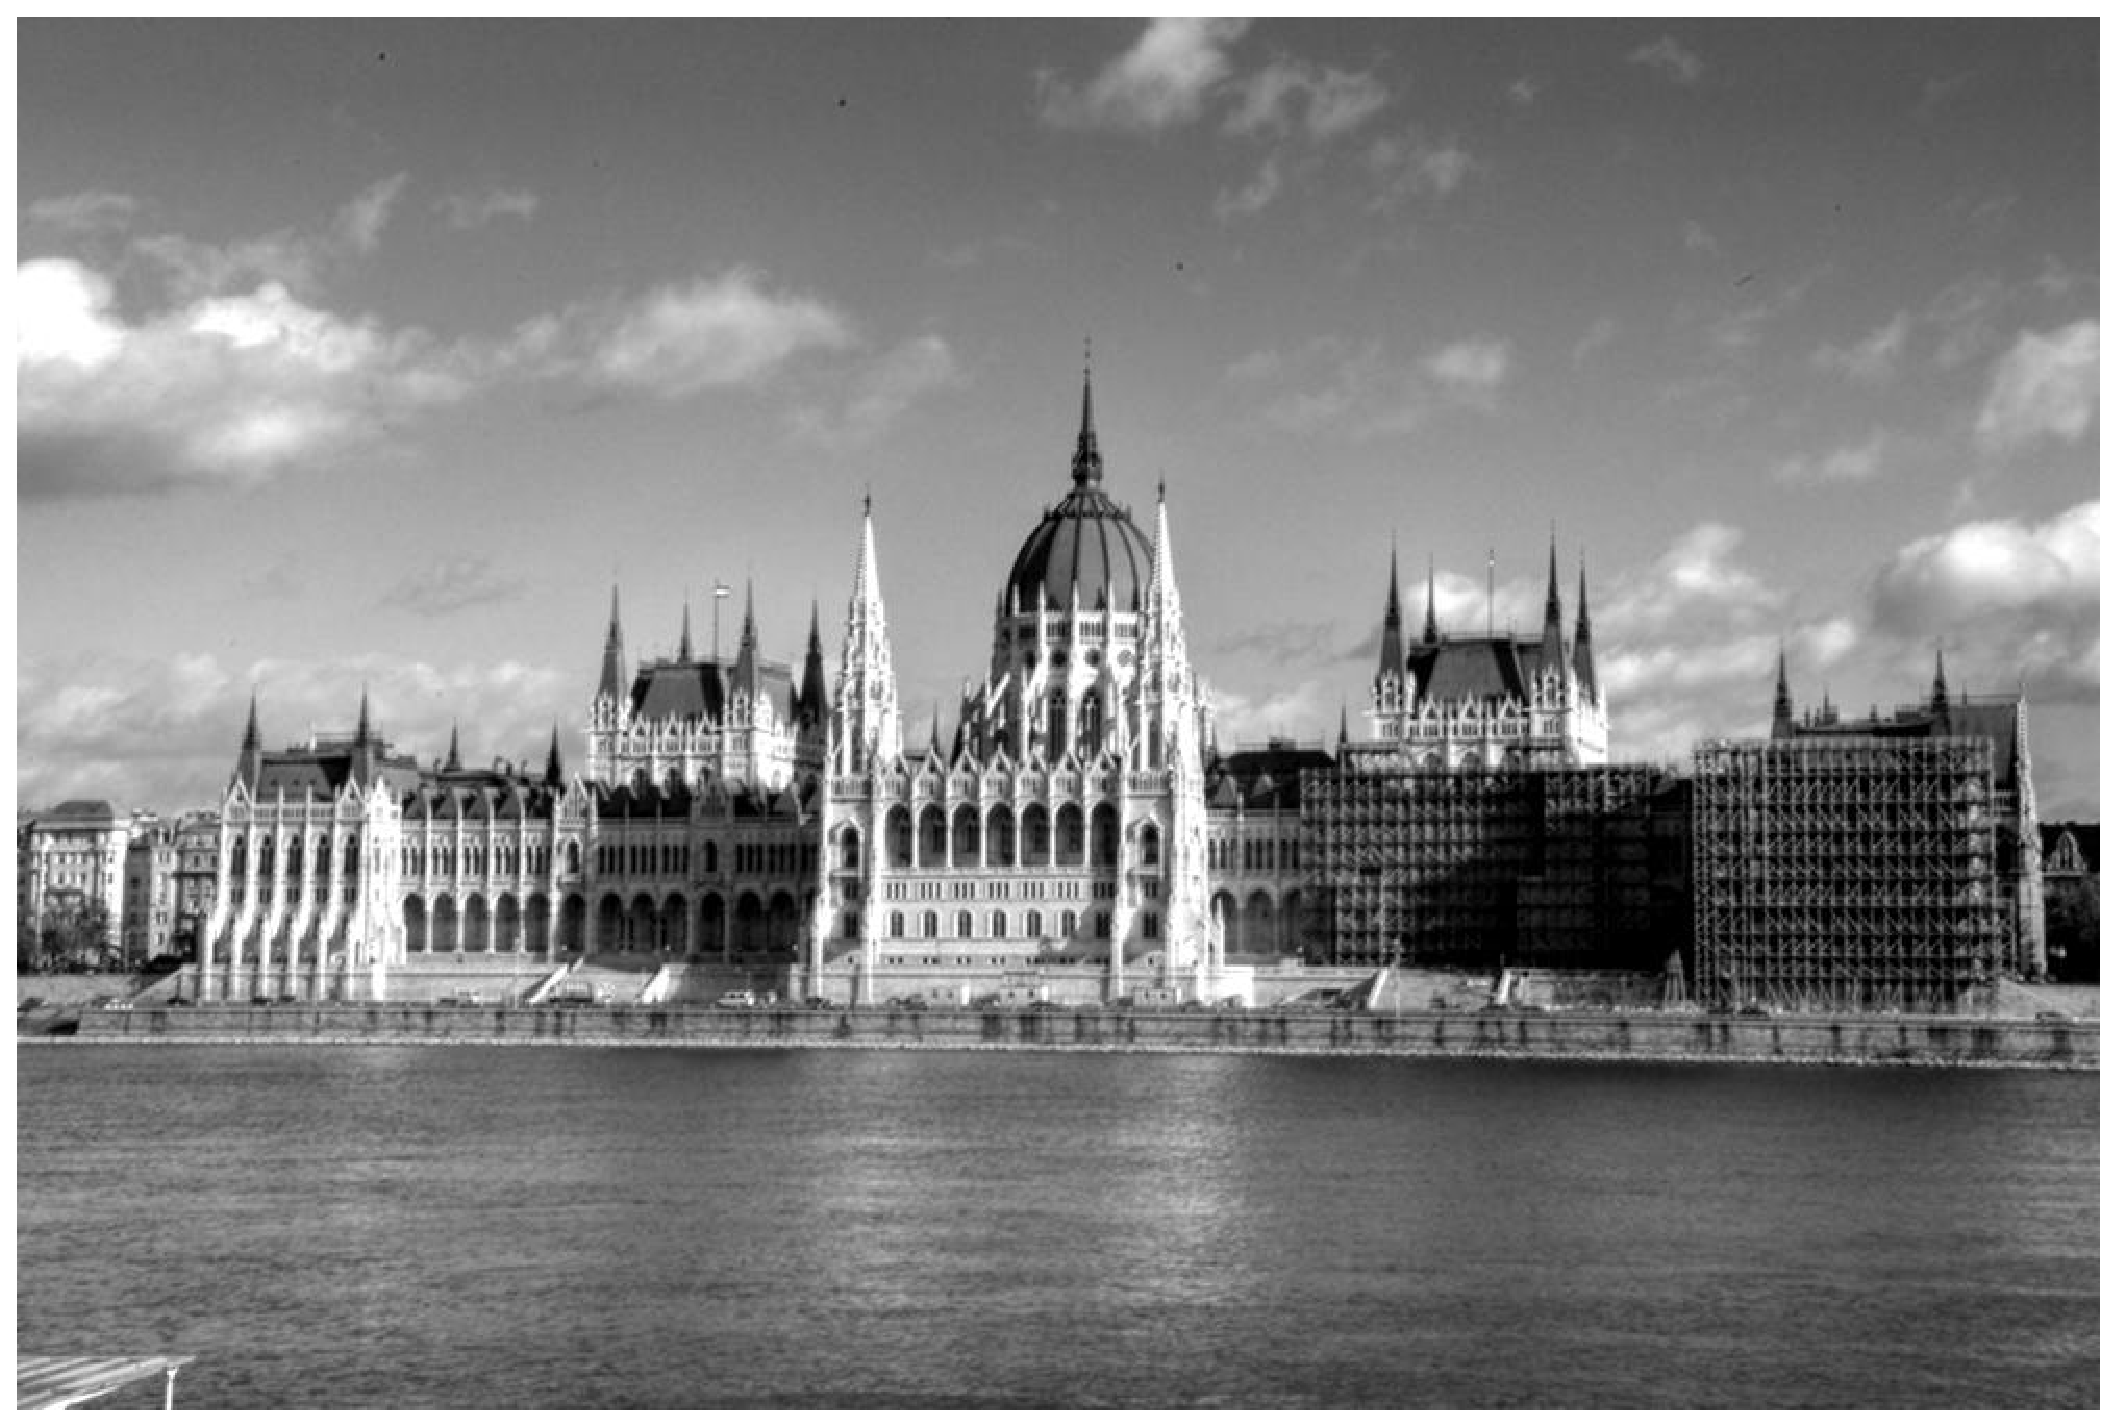
\includegraphics[width=0.24\textwidth]{newMethodBuda.eps}}
  \subfloat[][]{\label{figur:4d}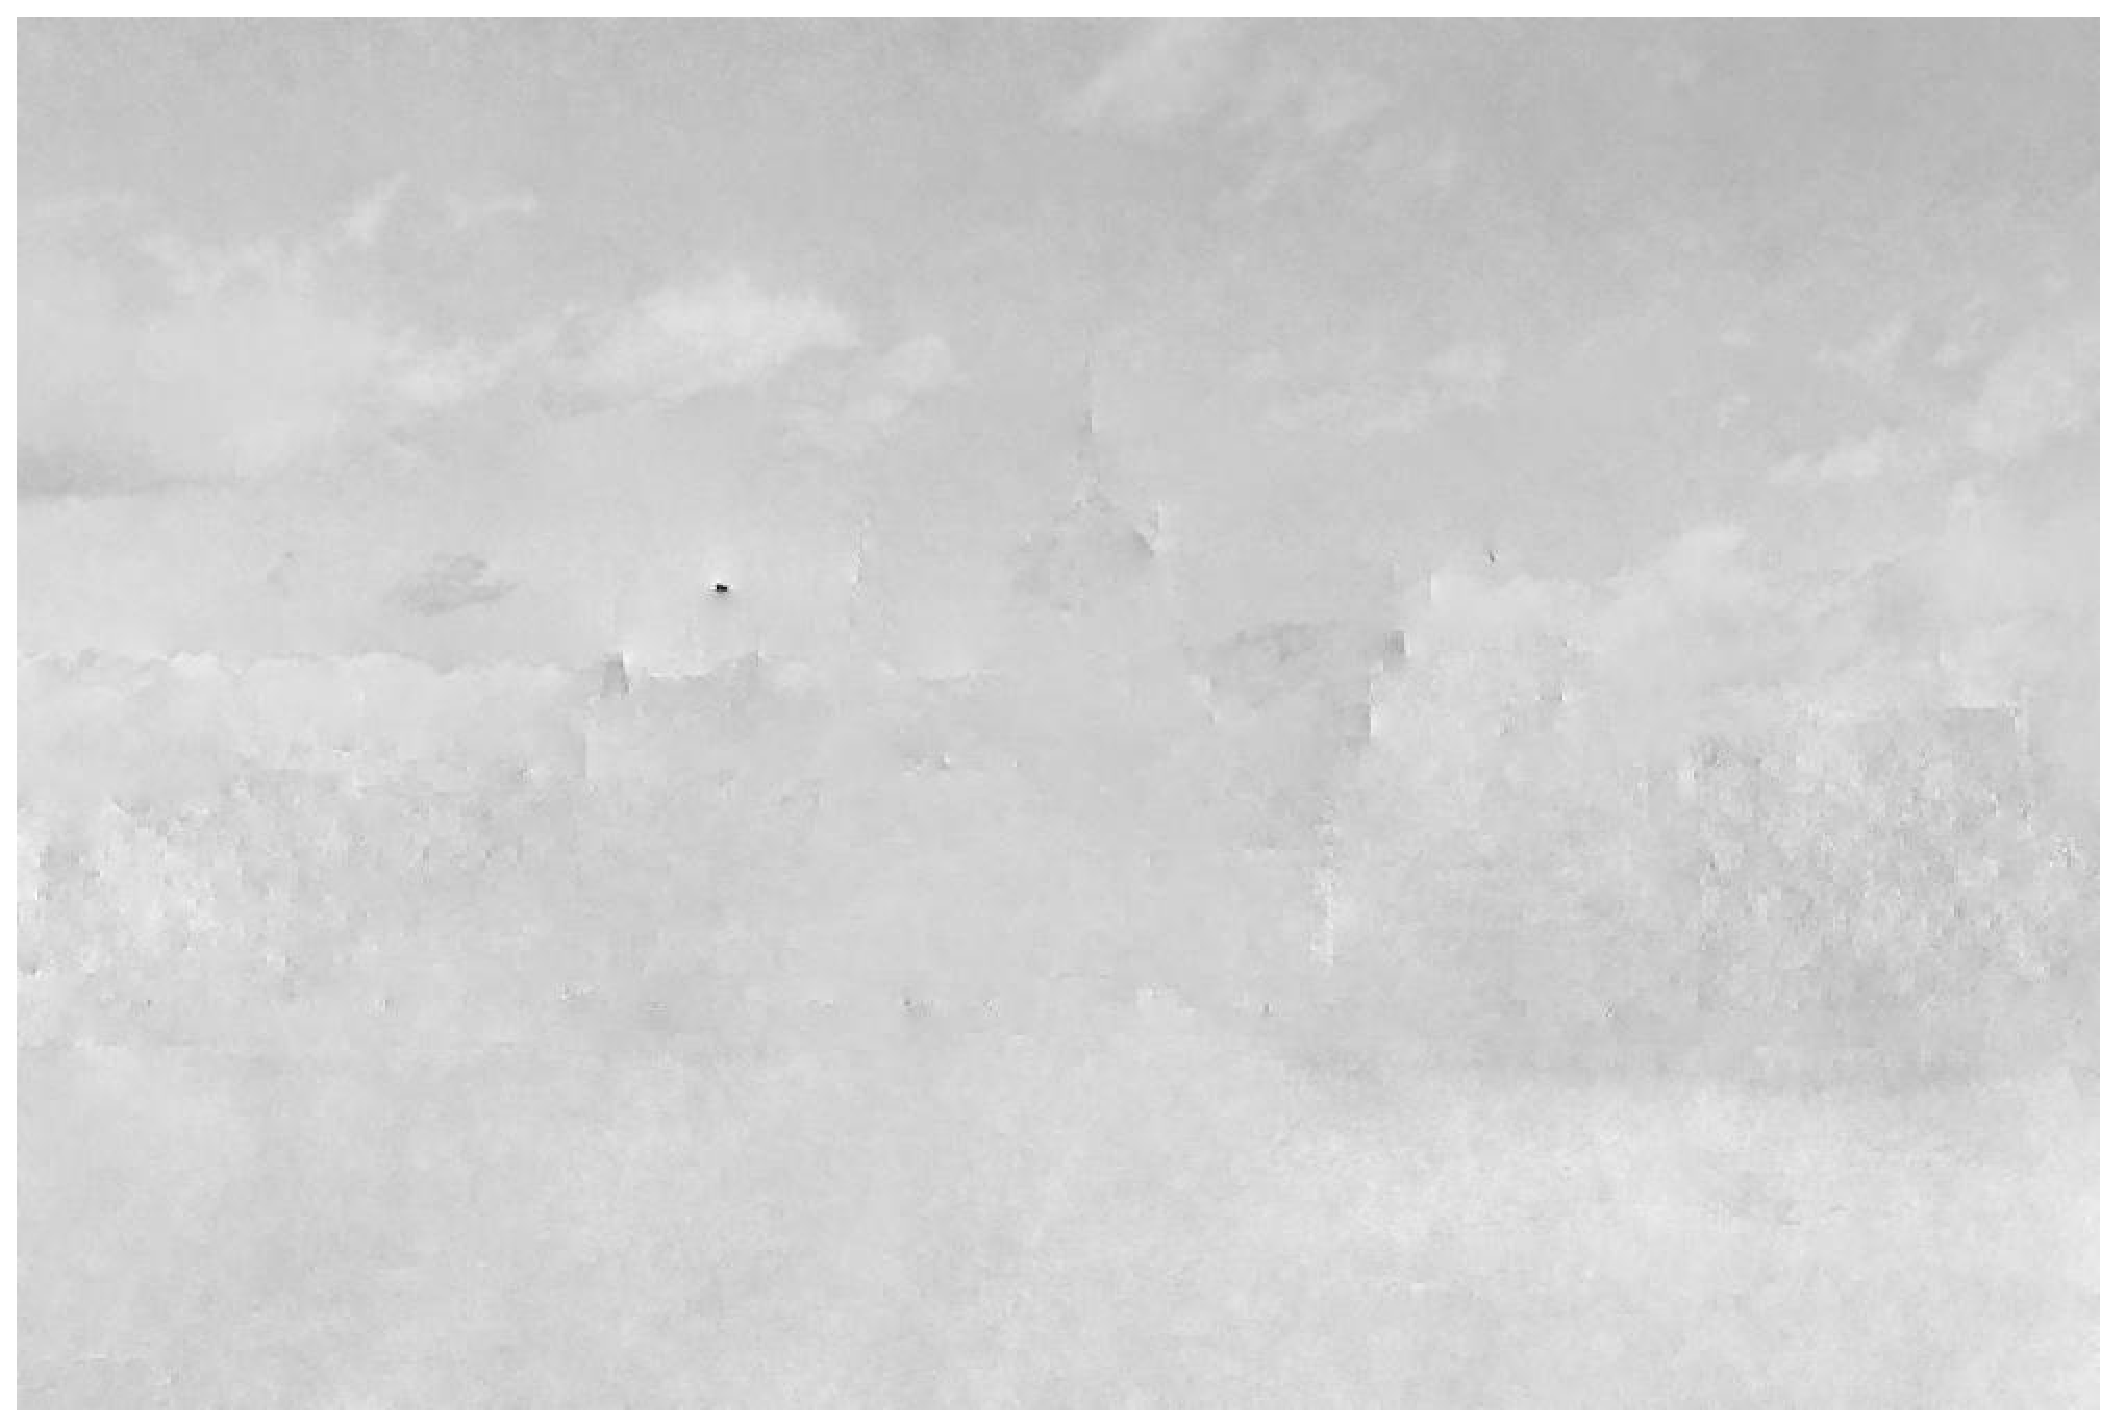
\includegraphics[width=0.24\textwidth]{newMethodBuda_rest.eps}}
\caption{Results of converting the Hungarian Parliament original photo~\ref{figur:4a} to grey using the luminance channel~\ref{figur:4b} and the proposed algorithm~\ref{figur:4c}. The results of integrating the leftover gradients are shown in~\ref{figur:4d}.}
\label{fig:4}
\end{figure}
\begin{figure}[t]  
  \centering
\psset{xunit=1.2cm,yunit=0.8cm}
\begin{pspicture}(-1,-1)(7,7)
\psgrid[gridcolor=gray,subgriddiv=0,gridwidth=0.4pt,gridlabels=0](0,0)(0,0)(6,7)
\pspolygon[linewidth=0.005](0,0)(0,7)(6,7)(6,0)
\rput(0, 0.11604){\color{blue}$\bigstar$}
\rput(1, 0.49292){\color{blue}$\bigstar$}
\rput(2, 0.95978){\color{blue}$\bigstar$}
\rput(3, 0.28835){\color{blue}$\bigstar$}
\rput(4, 0.56871){\color{blue}$\bigstar$}
\rput(5, 1.11858){\color{blue}$\bigstar$}
\rput(6, 6.42648){\color{blue}$\bigstar$}
\rput[r](-0.1,0){\scriptsize 0.0}%
\rput[r](-0.1,1){\scriptsize 0.1}%
\rput[r](-0.1,2){\scriptsize 0.2}%
\rput[r](-0.1,3){\scriptsize 0.3}%
\rput[r](-0.1,4){\scriptsize 0.4}%
\rput[r](-0.1,5){\scriptsize 0.5}%
\rput[r](-0.1,6){\scriptsize 0.6}%
\rput[r](-0.1,7){\scriptsize 0.7}%
\rput[B](0,-0.35){\scriptsize blue}%
\rput[B](1,-0.35){\scriptsize green}%
\rput[B](2,-0.35){\scriptsize cyan}%
\rput[B](3,-0.35){\scriptsize red}%
\rput[B](4,-0.35){\scriptsize magenta}%
\rput[B](5,-0.35){\scriptsize yellow}%
\rput[B](6,-0.35){\scriptsize white}%
\rput(3,-.84){Maximum gradient direction}
\rput{90}(-.6,3.5){Normalised count}
\end{pspicture}  
%{\includegraphics[width=0.47\textwidth]{gradients_buda2.eps}}
\caption{The percentage of maximum signed gradients for the Hungarian Parliament in different directions. Here white is luminance gradients and it is the direction in which all the colour values increase or decrease.}
\label{fig:4G}
\end{figure}
\section{Discussion} 
    
% Generated by IEEEtran.bst, version: 1.12 (2007/01/11)
\begin{thebibliography}{1}
\providecommand{\url}[1]{#1}
\csname url@samestyle\endcsname
\providecommand{\newblock}{\relax}
\providecommand{\bibinfo}[2]{#2}
\providecommand{\BIBentrySTDinterwordspacing}{\spaceskip=0pt\relax}
\providecommand{\BIBentryALTinterwordstretchfactor}{4}
\providecommand{\BIBentryALTinterwordspacing}{\spaceskip=\fontdimen2\font plus
\BIBentryALTinterwordstretchfactor\fontdimen3\font minus
  \fontdimen4\font\relax}
\providecommand{\BIBforeignlanguage}[2]{{%
\expandafter\ifx\csname l@#1\endcsname\relax
\typeout{** WARNING: IEEEtran.bst: No hyphenation pattern has been}%
\typeout{** loaded for the language `#1'. Using the pattern for}%
\typeout{** the default language instead.}%
\else
\language=\csname l@#1\endcsname
\fi
#2}}
\providecommand{\BIBdecl}{\relax}
\BIBdecl

\bibitem{Wei02heightfrom}
T.~Wei and R.~Klette, ``Height from gradient using surface curvature and area
  constraints,'' in \emph{In 3rd Indian Conference on Computer Vision, Graphics
  and Image Processing}.\hskip 1em plus 0.5em minus 0.4em\relax Ahmedabad,
  2002.

\bibitem{socolinsky1999new}
D.~A. Socolinsky and L.~B. Wolff, ``A new visualization paradigm for
  multispectral imagery and data fusion,'' in \emph{Proceedings. 1999 IEEE
  Computer Society Conference on Computer Vision and Pattern Recognition (Cat.
  No PR00149)}, vol.~1.\hskip 1em plus 0.5em minus 0.4em\relax IEEE, 1999, pp.
  319--324.

\bibitem{farup2018colour}
I.~Farup, M.~Pedersen, and A.~Alsam, ``Colour-to-greyscale image conversion by
  linear anisotropic diffusion of perceptual colour metrics,'' in \emph{2018
  Colour and Visual Computing Symposium (CVCS)}.\hskip 1em plus 0.5em minus
  0.4em\relax IEEE, 2018, pp. 1--6.

\bibitem{Alsam_Drew_FastColour2Grey_2008}
A.~Alsam and M.~S. Drew, ``Fastcolour2grey,'' \emph{16th Color Imaging
  Conference: Color, Science, Systems and Applications, Society for Imaging
  Science \& Technology (IS\&T)/Society for Information Display (SID) joint
  conference, Portland, Oregon.}, pp. 342--346, 2008.

\bibitem{Alsam2009_FastMultispectral2Gray}
------, ``Fast multispectral2gray,'' \emph{Journal of Imaging Science and
  Technology}, vol.~53, no.~6, p. 060401, Nov-Dec 2009.

\bibitem{Minkowski:03}
\BIBentryALTinterwordspacing
H.~Minkowski, ``Volumen und {O}berfl\"{a}che,'' \emph{Math. Ann.}, vol.~57,
  no.~4, pp. 447--495, 1903. [Online]. Available:
  \url{https://doi.org/10.1007/BF01445180}
\BIBentrySTDinterwordspacing

\bibitem{Mackiewicz:19}
\BIBentryALTinterwordspacing
M.~Mackiewicz, H.~J. Rivertz, and G.~Finlayson, ``Spherical sampling methods
  for the calculation of metamer mismatch volumes,'' \emph{J. Opt. Soc. Am. A},
  vol.~36, no.~1, pp. 96--104, Jan 2019. [Online]. Available:
  \url{http://josaa.osa.org/abstract.cfm?URI=josaa-36-1-96}
\BIBentrySTDinterwordspacing

\bibitem{Chellappa:05}
A.~{Agrawal}, R.~{Chellappa}, and R.~{Raskar}, ``An algebraic approach to
  surface reconstruction from gradient fields,'' in \emph{Tenth IEEE
  International Conference on Computer Vision (ICCV'05) Volume 1}, vol.~1, Oct 2005, pp. 174--181 Vol. 1.\\[-2mm]

\end{thebibliography}

\end{document}

